\PassOptionsToPackage{unicode=true}{hyperref} % options for packages loaded elsewhere
\PassOptionsToPackage{hyphens}{url}
%
\documentclass[]{article}
\usepackage{lmodern}
\usepackage{amssymb,amsmath}
\usepackage{ifxetex,ifluatex}
\usepackage{fixltx2e} % provides \textsubscript
\ifnum 0\ifxetex 1\fi\ifluatex 1\fi=0 % if pdftex
  \usepackage[T1]{fontenc}
  \usepackage[utf8]{inputenc}
  \usepackage{textcomp} % provides euro and other symbols
\else % if luatex or xelatex
  \usepackage{unicode-math}
  \defaultfontfeatures{Ligatures=TeX,Scale=MatchLowercase}
\fi
% use upquote if available, for straight quotes in verbatim environments
\IfFileExists{upquote.sty}{\usepackage{upquote}}{}
% use microtype if available
\IfFileExists{microtype.sty}{%
\usepackage[]{microtype}
\UseMicrotypeSet[protrusion]{basicmath} % disable protrusion for tt fonts
}{}
\IfFileExists{parskip.sty}{%
\usepackage{parskip}
}{% else
\setlength{\parindent}{0pt}
\setlength{\parskip}{6pt plus 2pt minus 1pt}
}
\usepackage{hyperref}
\hypersetup{
            pdftitle={Flujo de análisis en clasificación supervisada},
            pdfauthor={Laura Rodríguez Navas},
            pdfborder={0 0 0},
            breaklinks=true}
\urlstyle{same}  % don't use monospace font for urls
\usepackage[margin=1in]{geometry}
\usepackage{color}
\usepackage{tcolorbox}
\usepackage{fancyvrb}
\newcommand{\VerbBar}{|}
\newcommand{\VERB}{\Verb[commandchars=\\\{\}]}
\DefineVerbatimEnvironment{Highlighting}{Verbatim}{commandchars=\\\{\}}
% Add ',fontsize=\small' for more characters per line
\usepackage{framed}
\definecolor{shadecolor}{RGB}{248,248,248}
\newenvironment{Shaded}{\begin{snugshade}}{\end{snugshade}}
\newcommand{\AlertTok}[1]{\textcolor[rgb]{0.94,0.16,0.16}{#1}}
\newcommand{\AnnotationTok}[1]{\textcolor[rgb]{0.56,0.35,0.01}{\textbf{\textit{#1}}}}
\newcommand{\AttributeTok}[1]{\textcolor[rgb]{0.77,0.63,0.00}{#1}}
\newcommand{\BaseNTok}[1]{\textcolor[rgb]{0.00,0.00,0.81}{#1}}
\newcommand{\BuiltInTok}[1]{#1}
\newcommand{\CharTok}[1]{\textcolor[rgb]{0.31,0.60,0.02}{#1}}
\newcommand{\CommentTok}[1]{\textcolor[rgb]{0.56,0.35,0.01}{\textit{#1}}}
\newcommand{\CommentVarTok}[1]{\textcolor[rgb]{0.56,0.35,0.01}{\textbf{\textit{#1}}}}
\newcommand{\ConstantTok}[1]{\textcolor[rgb]{0.00,0.00,0.00}{#1}}
\newcommand{\ControlFlowTok}[1]{\textcolor[rgb]{0.13,0.29,0.53}{\textbf{#1}}}
\newcommand{\DataTypeTok}[1]{\textcolor[rgb]{0.13,0.29,0.53}{#1}}
\newcommand{\DecValTok}[1]{\textcolor[rgb]{0.00,0.00,0.81}{#1}}
\newcommand{\DocumentationTok}[1]{\textcolor[rgb]{0.56,0.35,0.01}{\textbf{\textit{#1}}}}
\newcommand{\ErrorTok}[1]{\textcolor[rgb]{0.64,0.00,0.00}{\textbf{#1}}}
\newcommand{\ExtensionTok}[1]{#1}
\newcommand{\FloatTok}[1]{\textcolor[rgb]{0.00,0.00,0.81}{#1}}
\newcommand{\FunctionTok}[1]{\textcolor[rgb]{0.00,0.00,0.00}{#1}}
\newcommand{\ImportTok}[1]{#1}
\newcommand{\InformationTok}[1]{\textcolor[rgb]{0.56,0.35,0.01}{\textbf{\textit{#1}}}}
\newcommand{\KeywordTok}[1]{\textcolor[rgb]{0.13,0.29,0.53}{\textbf{#1}}}
\newcommand{\NormalTok}[1]{#1}
\newcommand{\OperatorTok}[1]{\textcolor[rgb]{0.81,0.36,0.00}{\textbf{#1}}}
\newcommand{\OtherTok}[1]{\textcolor[rgb]{0.56,0.35,0.01}{#1}}
\newcommand{\PreprocessorTok}[1]{\textcolor[rgb]{0.56,0.35,0.01}{\textit{#1}}}
\newcommand{\RegionMarkerTok}[1]{#1}
\newcommand{\SpecialCharTok}[1]{\textcolor[rgb]{0.00,0.00,0.00}{#1}}
\newcommand{\SpecialStringTok}[1]{\textcolor[rgb]{0.31,0.60,0.02}{#1}}
\newcommand{\StringTok}[1]{\textcolor[rgb]{0.31,0.60,0.02}{#1}}
\newcommand{\VariableTok}[1]{\textcolor[rgb]{0.00,0.00,0.00}{#1}}
\newcommand{\VerbatimStringTok}[1]{\textcolor[rgb]{0.31,0.60,0.02}{#1}}
\newcommand{\WarningTok}[1]{\textcolor[rgb]{0.56,0.35,0.01}{\textbf{\textit{#1}}}}
\usepackage{graphicx,grffile}
\makeatletter
\def\maxwidth{\ifdim\Gin@nat@width>\linewidth\linewidth\else\Gin@nat@width\fi}
\def\maxheight{\ifdim\Gin@nat@height>\textheight\textheight\else\Gin@nat@height\fi}
\makeatother
% Scale images if necessary, so that they will not overflow the page
% margins by default, and it is still possible to overwrite the defaults
% using explicit options in \includegraphics[width, height, ...]{}
\setkeys{Gin}{width=\maxwidth,height=\maxheight,keepaspectratio}
\setlength{\emergencystretch}{3em}  % prevent overfull lines
\providecommand{\tightlist}{%
  \setlength{\itemsep}{0pt}\setlength{\parskip}{0pt}}
\setcounter{secnumdepth}{0}
% Redefines (sub)paragraphs to behave more like sections
\ifx\paragraph\undefined\else
\let\oldparagraph\paragraph
\renewcommand{\paragraph}[1]{\oldparagraph{#1}\mbox{}}
\fi
\ifx\subparagraph\undefined\else
\let\oldsubparagraph\subparagraph
\renewcommand{\subparagraph}[1]{\oldsubparagraph{#1}\mbox{}}
\fi

% set default figure placement to htbp
\makeatletter
\def\fps@figure{htbp}
\makeatother

\usepackage{etoolbox}
\makeatletter
\providecommand{\subtitle}[1]{% add subtitle to \maketitle
  \apptocmd{\@title}{\par {\large #1 \par}}{}{}
}
\makeatother

\title{Flujo de análisis en clasificación supervisada}
\providecommand{\subtitle}[1]{}
\subtitle{Métodos supervisados}
\author{Laura Rodríguez Navas}
\date{Septiembre 2020}

\begin{document}
\maketitle

{
\setcounter{tocdepth}{3}
\renewcommand{\contentsname}{Contenido}
\tableofcontents
}
\newpage

Empezamos por cargar a nuestro espacio de trabajo los paquetes que
usaremos:

\begin{itemize}
\tightlist
\item
  \textbf{tidyverse}, engloba otros paquetes (\textbf{dplyr},
  \textbf{tidyr}, \textbf{ggplot}, etc.) que facilitan en gran medida el
  análisis exploratorio de los datos.
\item
  \textbf{tm}, específico para minería de textos.
\item
  \textbf{irlba}, específico para la \emph{Descomposición de Valores
  Singulares (SVD)} de matrices muy grandes.
\item
  \textbf{caret}, para realizar tareas de clasificación y regresión.
\item
  \textbf{doParallel}, proporciona computación paralela.
\item
  \textbf{syuzhet}, específico para la extracción de sentimientos (información subjetiva) de
  textos.
\item
  \textbf{ggcorrplot}, muestra visualizaciones gráficas de matrices de
  correlación usando \textbf{ggplot2}.
\end{itemize}

\vspace{3mm}

\begin{Shaded}
\begin{Highlighting}[]
\KeywordTok{library}\NormalTok{(tidyverse)}
\KeywordTok{library}\NormalTok{(tm)}
\KeywordTok{library}\NormalTok{(irlba)}
\KeywordTok{library}\NormalTok{(caret)}
\KeywordTok{library}\NormalTok{(doParallel)}
\KeywordTok{library}\NormalTok{(syuzhet)}
\KeywordTok{library}\NormalTok{(ggcorrplot)}
\end{Highlighting}
\end{Shaded}

\hypertarget{anuxe1lisis-exploratorio-de-los-datos}{%
\section{Análisis exploratorio de los
datos}\label{anuxe1lisis-exploratorio-de-los-datos}}

Antes de entrenar un modelo predictivo, o incluso antes de realizar
cualquier cálculo con un nuevo conjunto de datos, es muy importante
realizar una exploración descriptiva de los datos. Este proceso nos
permite entender mejor que información contienen cada variable, detectar
posibles errores, etc. además, puede dar pistas sobre qué variables no
son adecuadas para predecir un modelo.

Acorde a la realización del ejercicio propuesto se ha elegido la
competición en Kaggle: \emph{Real or Not? NLP with Disaster Tweets}.
El dataset de la competición se puede encontrar en el siguiente \href{https://www.kaggle.com/c/nlp-getting-started/data}{\color{blue}{enlace}}. Este dataset,
con 10.876 instancias, contiene 4 variables explicativas: \textbf{id},
\textbf{keyword}, \textbf{location} y \textbf{text}, y dos valores en la
variable clase \textbf{target} (0 y 1). Como observaremos la
variable clase es binaria, así que, durante este ejercicio vamos a
crear un modelo de \emph{clasificación binaria}. El objetivo de este
modelo será predecir si dado un tweet, éste trata sobre un desastre real
o no. Si un tweet trata sobre un desastre real, se predice un 1. Si no,
se predice un 0.

\begin{tcolorbox}
La \textbf{clasificación binaria} es un tipo de clasificación en el que tan solo se pueden asignar dos clases diferentes (0 o 1).	
\end{tcolorbox}

La métrica de evaluación esperada por la competición de Kaggle es \textbf{F1}. Para más información consultar el siguiente \href{https://www.kaggle.com/c/nlp-getting-started/overview/evaluation}{\color{blue}enlace}. Se calcula de la siguiente manera:

\vspace{3mm}

\begin{center}
	F1 = 2 * $\dfrac{precision * recall}{precision + recall}$
\end{center}

donde:

\begin{center}	
	precision = $\dfrac{TP}{TP + FP}$
	
	recall = $\dfrac{TP}{TP + FN}$
\end{center}

\begin{itemize}
	\item True Positive (TP)
	\item False Positive (FP)
	\item False Negative (FN)
\end{itemize}

La partición inicial train-test, no se tiene que realizar, ya que las
instancias de train y test ya vienen definidas en el dataset de la
competición de Kaggle. Solo tendremos que descargar a nuestro espacio de trabajo los ficheros
\textbf{train.csv} y \textbf{test.csv} des del siguiente 
\href{https://www.kaggle.com/c/nlp-getting-started/data}{\color{blue}enlace}).

Cargamos a nuestro espacio de trabajo los conjuntos de datos de train y test que hemos descargado con la función \textbf{read.csv()}, renombrando los valores perdidos como \textbf{NA} para que los podamos tratar más adelante. 

Además, mostramos las dimensiones de los conjuntos de datos de train y test usando la función \textbf{dim()}. Esta función nos mostrará el número total de observaciones y de variables de cada conjunto de datos.

\vspace{3mm}

\begin{Shaded}
\begin{Highlighting}[]
\NormalTok{train <-}\StringTok{ }\KeywordTok{read.csv}\NormalTok{(}\StringTok{"train.csv"}\NormalTok{, }\DataTypeTok{na.strings=}\KeywordTok{c}\NormalTok{(}\StringTok{""}\NormalTok{, }\StringTok{"NA"}\NormalTok{))}
\NormalTok{test <-}\StringTok{ }\KeywordTok{read.csv}\NormalTok{(}\StringTok{"test.csv"}\NormalTok{, }\DataTypeTok{na.strings=}\KeywordTok{c}\NormalTok{(}\StringTok{""}\NormalTok{, }\StringTok{"NA"}\NormalTok{))}
\KeywordTok{dim}\NormalTok{(train)}
\end{Highlighting}
\end{Shaded}

\begin{verbatim}
## [1] 7613    5
\end{verbatim}

\begin{Shaded}
\begin{Highlighting}[]
\KeywordTok{dim}\NormalTok{(test)}
\end{Highlighting}
\end{Shaded}

\begin{verbatim}
## [1] 3263    4
\end{verbatim}

Vemos que el conjunto de datos de train contiene 7613 instancias y el
conjunto de datos de test contiene 3263 instancias. Cada instancia
contiene las siguientes variables:

\begin{itemize}
\tightlist
\item
  \textbf{id}: un identificador único para cada tweet.
\item
  \textbf{keyword}: una palabra clave del tweet.
\item
  \textbf{location}: la ubicación desde la que se envió el tweet.
\item
  \textbf{text}: el texto del tweet.
\item
  \textbf{target}: solo en el conjunto de datos de train porqué es la
  variable clase, la variable a predecir. Indica si un tweet corresponde a un
  desastre real (1) o no (0).
\end{itemize}

El conjunto de datos de train:

\begin{verbatim}
## 'data.frame':    7613 obs. of  5 variables:
##  $ id      : int  1 4 5 6 7 8 10 13 14 15 ...
##  $ keyword : chr  NA NA NA NA ...
##  $ location: chr  NA NA NA NA ...
##  $ text    : chr  "Our Deeds are the Reason of this #earthquake May ALLAH Forgive "..
##  $ target  : int  1 1 1 1 1 1 1 1 1 1 ...
\end{verbatim}

El conjunto de datos de test:

\begin{verbatim}
## 'data.frame':    3263 obs. of  4 variables:
##  $ id      : int  0 2 3 9 11 12 21 22 27 29 ...
##  $ keyword : chr  NA NA NA NA ...
##  $ location: chr  NA NA NA NA ...
##  $ text    : chr  "Just happened a terrible car crash" "Heard about #earthquake is"..
\end{verbatim}

\hypertarget{variable-target}{%
\subsection{\texorpdfstring{Variable
\emph{target}}{Variable target}}\label{variable-target}}

Como acabamos de comentar en la sección anterior, la variable \textbf{target} es la variable clase y la variable a
predecir. La variable es de tipo cuantitativa, concretamente de tipo entero, y conviene
transformarla para que sea una variable de tipo cualitativa (categórica). 

Para transformar la variable a predecir en una variable categórica usamos la función \textbf{as.factor()}. Esto lo hacemos para evitar errores futuros, y además se re-codifica para que sus dos posibles valores sean ``Yes'' y ``No''.

\vspace{3mm}

\begin{Shaded}
\begin{Highlighting}[]
\NormalTok{train}\OperatorTok{$}\NormalTok{target <-}\StringTok{ }\KeywordTok{as.factor}\NormalTok{(}\KeywordTok{ifelse}\NormalTok{(train}\OperatorTok{$}\NormalTok{target }\OperatorTok{==}\StringTok{ }\DecValTok{0}\NormalTok{, }\StringTok{"No"}\NormalTok{, }\StringTok{"Yes"}\NormalTok{))}
\KeywordTok{ggplot}\NormalTok{(train, }\KeywordTok{aes}\NormalTok{(}\DataTypeTok{x=}\NormalTok{target)) }\OperatorTok{+}\StringTok{ }\KeywordTok{geom_bar}\NormalTok{(}\KeywordTok{aes}\NormalTok{(}\DataTypeTok{fill=}\NormalTok{target))}
\end{Highlighting}
\end{Shaded}

\renewcommand{\figurename}{Figura}

\begin{figure}
	\begin{center}
		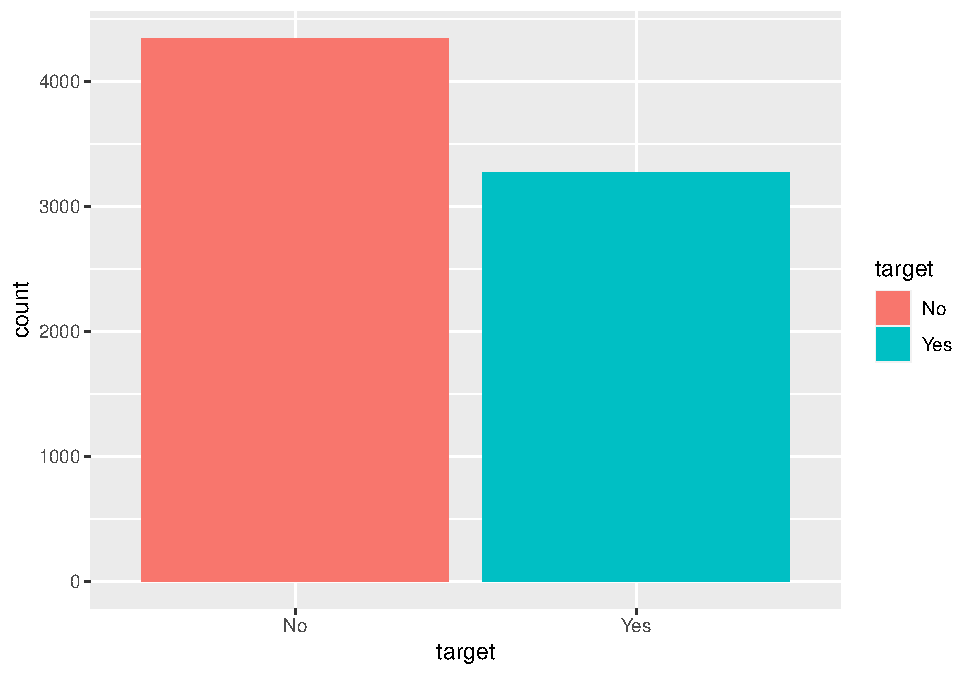
\includegraphics[width=0.7\linewidth]{document_files/figure-latex/unnamed-chunk-4-1} 
		\caption{distribución de la variable \textbf{target}.}
		\label{fig: distribución de la variable target}
	\end{center}
\end{figure}

Cuando se quiere crear un modelo de predicción, es muy importante estudiar la distribución de
la variable clase, en este caso la variable a predecir, ya que, a fin de cuentas, es lo que nos interesa
predecir.

Gráficamente (ver Figura \ref{fig: distribución de la variable target}) observamos que la distribución de la variable a predecir no está muy sesgada y que está relativamente equilibrada. Aunque si nos fijamos hay menos tweets que se refieren a desastres reales (columna "Yes"). Así, la clase ``Yes'' representaría a la clase minoritaria y la clase "No", a la clase mayoritaria. Tampoco parece que presente un problema notable de \emph{desequilibrio de clases}, porqué contamos con muchas observaciones de la clase minoritaria.

\begin{tcolorbox}
	Al enfrentarse a la situación de crear un modelo de clasificación binaria es habitual que las clases no se encuentren balanceadas. Esto es, el número de observaciones para una de las clases es inferior a la otra. Cuando el desequilibrio es pequeño, esto no supone un problema, pero cuando el desequilibrio es grande es un problema para la mayoría de los modelos de clasificación. Esta situación se conoce como el \textbf{problema del desequilibrio de clases}.
\end{tcolorbox}

\vspace{3mm}

\begin{Shaded}
\begin{Highlighting}[]
\KeywordTok{sum}\NormalTok{(train}\OperatorTok{$}\NormalTok{target }\OperatorTok{==}\StringTok{ "Yes"}\NormalTok{) }\OperatorTok{/}\StringTok{ }\KeywordTok{dim}\NormalTok{(train)[}\DecValTok{1}\NormalTok{] }\OperatorTok{*}\StringTok{ }\DecValTok{100}
\end{Highlighting}
\end{Shaded}

\begin{verbatim}
## [1] 42.96598
\end{verbatim}

\begin{Shaded}
\begin{Highlighting}[]
\KeywordTok{sum}\NormalTok{(train}\OperatorTok{$}\NormalTok{target }\OperatorTok{==}\StringTok{ "No"}\NormalTok{) }\OperatorTok{/}\StringTok{ }\KeywordTok{dim}\NormalTok{(train)[}\DecValTok{1}\NormalTok{] }\OperatorTok{*}\StringTok{ }\DecValTok{100}
\end{Highlighting}
\end{Shaded}

\begin{verbatim}
## [1] 57.03402
\end{verbatim}

Concretamente, el 57\% de los tweets corresponden a desastres no reales, y aproximadamente el 43\% corresponden a desastres reales. Para que el modelo predictivo que crearemos nos sea útil, tendremos que intentar superar ese porcentaje mínimo del 57\% de la clase mayoritaria.

Como el objetivo del ejercicio es predecir que tweets pertenecen o no a un desastre real, lo que haremos a continuación, es analizar las variables explicativas del conjunto de datos de train en relación a la variable a predecir \textbf{target}. De este análisis se podrán extraer ideas sobre que variables están más relacionadas con los desastres reales.

\hypertarget{variable-keyword}{%
\subsection{\texorpdfstring{Variable
\emph{keyword}}{Variable keyword}}\label{variable-keyword}}

La variable explicativa \textbf{keyword} representa una palabra clave en cada tweet. Vemos las 10 primeras del conjunto de datos de train usando las funciones \textbf{select()}, \textbf{unique()} para no ver las variables repetidas, y \textbf{head()} donde le decimos que cantidad de variables queremos ver.

\vspace{3mm}

\begin{Shaded}
\begin{Highlighting}[]
\NormalTok{train }\OperatorTok\StringTok{ }\KeywordTok{select}\NormalTok{(keyword) }\OperatorTok\StringTok{ }\KeywordTok{unique}\NormalTok{() }\OperatorTok\StringTok{ }\KeywordTok{head}\NormalTok{(}\DecValTok{10}\NormalTok{)}
\end{Highlighting}
\end{Shaded}

\begin{verbatim}
##                 keyword
## 1                  <NA>
## 32               ablaze
## 68             accident
## 103          aftershock
## 137 airplane%20accident
## 172           ambulance
## 210         annihilated
## 244        annihilation
## 273          apocalypse
## 305          armageddon
\end{verbatim}

Nuestro interés en la variable \textbf{keyword}, dentro del análisis exploratorio, es ver si existen correlaciones entre ella y la variable a predecir \textbf{target}. Para ello, y como estamos delante un ejercicio de \href{https://es.wikipedia.org/wiki/Procesamiento_de_lenguajes_naturales}{\color{blue}Procesamiento del Lenguaje Natural}, realizaremos un \textbf{análisis de sentimientos}.

\begin{tcolorbox}
	El \textbf{análisis de sentimientos} es una técnica de \href{https://en.wikipedia.org/wiki/Machine_learning}{\color{blue}Machine Learning},
	basada en el Procesamiento del Lenguaje Natural, que pretende obtener información subjetiva de una
	serie de textos.
\end{tcolorbox}

Para el análisis de sentimientos usamos los paquetes: \textbf{syuzhet}, \textbf{ggcorrplot} y \textbf{doParallel}.

\begin{itemize}
\tightlist
\item
  \textbf{syuzhet} cuenta con la función
  \textbf{get\_nrc\_sentiment()} que calculará la presencia de los
  diferentes sentimientos dado un conjunto de palabras clave (variable \textbf{keyword}). 
  
  Los argumentos de esta función son:
  
  \vspace{2mm}

  \begin{itemize}
  \tightlist
  \item
    \textbf{char\_v}: un vector de caracteres que en este caso contendrá
    todas las palabras clave.
  \item
    \textbf{language}: define el lenguaje. Como los tweets están en
    inglés, el lenguaje será inglés.
  \item
    \textbf{cl}: para el análisis en paralelo. Es un argumento opcional, pero en este
    caso se usará porqué hay muchas palabras clave.
  \end{itemize}

\vspace{3mm}

\item
  \textbf{doParallel} cuenta con las funciones:
  
  \vspace{2mm}

  \begin{itemize}
  \tightlist
  \item
    \textbf{makePSOCKcluster()}: crea un clúster de sockets paralelos y inicia la computación paralela con estrategia secuencial.
  \item
    \textbf{registerDoParallel()}: registra el número de \emph{cores} que
    usará el clúster creado.
  \item
    \textbf{stopCluster()}: detiene la computación paralela.
  \end{itemize}
\end{itemize}

La computación paralela la usaremos en muchas de las ejecuciones de este ejercicio ya que nos encontramos delante de un problema de \textbf{alta dimensionalidad}. Eso es, que la dimensionalidad de nuestro dataset es tan elevada que puede reducir drásticamente la eficiencia de los modelos de clasificación supervisada que entrenaremos, además de producir un alto coste computacional.

Para solucionar el problema de la alta dimensionalidad de los datos, se realiza una \textbf{reducción de la dimensionalidad} (reducción del número de variables). La aplicaremos en este ejercicio, pero más adelante. Durante este proceso usaremos técnicas de \textbf{selección de variables} y \textbf{extracción de características}.

El análisis de sentimientos de nuestro ejercicio, consiste en extraer los sentimientos de cada palabra clave, con la función \textbf{get\_nrc\_sentiment()}. Guardar los sentimientos en un nuevo conjunto de datos (\textbf{emotion.df}). Y finalmente calcular la matriz de correlaciones (ver Figura \ref{fig: matriz de correlaciones}). Para calcular i visualizar la matriz de correlaciones usamos los paquetes \textbf{cor} y \textbf{ggcorrplot}. Es muy importante volver a transformar la variable a predecir \textbf{target}, a variable de tipo cuantitativa, porqué sino no podremos crear la matriz.

Veremos que se usa la función \textbf{gsub()} para eliminar los guiones bajos de las palabras clave y el argumento \textbf{lab} en la función \textbf{ggcorrplot()} para visualizar los coeficientes de correlación.

\vspace{3mm}


\begin{Shaded}
\begin{Highlighting}[]
\NormalTok{cl <-}\StringTok{ }\KeywordTok{makePSOCKcluster}\NormalTok{(}\DecValTok{4}\NormalTok{, }\DataTypeTok{setup_strategy=}\StringTok{"sequential"}\NormalTok{)}
\KeywordTok{registerDoParallel}\NormalTok{(cl)}

\NormalTok{emotion.df <-}\StringTok{ }\KeywordTok{get_nrc_sentiment}\NormalTok{(}\DataTypeTok{char_v =} \KeywordTok{gsub}\NormalTok{(}\StringTok{"_"}\NormalTok{, }\StringTok{" "}\NormalTok{, train}\OperatorTok{$}\NormalTok{keyword), }
                                \DataTypeTok{language =} \StringTok{"english"}\NormalTok{, }\DataTypeTok{cl=}\NormalTok{cl)}

\NormalTok{emotion.df <-}\StringTok{ }\NormalTok{emotion.df }\OperatorTok\StringTok{ }\KeywordTok{data.frame}\NormalTok{(}\DataTypeTok{target =}\NormalTok{ train}\OperatorTok{$}\NormalTok{target)}

\NormalTok{emotion.df}\OperatorTok{$}\NormalTok{target <-}\StringTok{ }\KeywordTok{as.numeric}\NormalTok{(emotion.df}\OperatorTok{$}\NormalTok{target)}

\KeywordTok{cor}\NormalTok{(emotion.df) }\OperatorTok\StringTok{ }
\StringTok{  }\KeywordTok{ggcorrplot}\NormalTok{(}\DataTypeTok{lab =} \OtherTok{TRUE}\NormalTok{, }
             \DataTypeTok{title =} \StringTok{"Matriz de correlación entre }\CharTok{\textbackslash{}n}\StringTok{keyword y target"}\NormalTok{,}
             \DataTypeTok{legend.title =} \StringTok{"correlation"}\NormalTok{)}
\end{Highlighting}
\end{Shaded}

\begin{figure}
	\begin{center}
		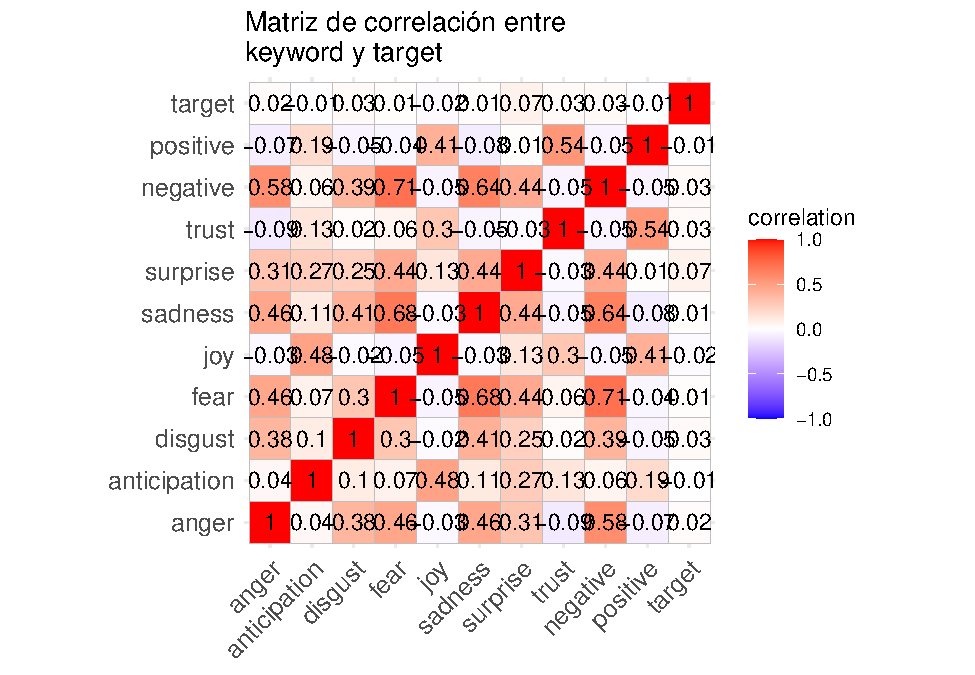
\includegraphics[width=1\linewidth]{document_files/figure-latex/unnamed-chunk-7-1} 
		\caption{matriz de correlaciones.}
		\label{fig: matriz de correlaciones}
	\end{center}
\end{figure}

\begin{Shaded}
\begin{Highlighting}[]
\KeywordTok{stopCluster}\NormalTok{(cl)}
\end{Highlighting}
\end{Shaded}

\newpage

Parece que al observar la matriz de correlaciones, existe una correlación nula entre las variables \textbf{keyword} y \textbf{target}. Si lo revisamos con mayor detalle, podemos observar que la mayoría de las
palabras clave no tienen un sentimiento positivo asociado, muchos de sus coeficientes se encuentran dentro del umbral: (-1.0, 0.5). Las palabras clave asociadas a un sentimiento se asocian negativamente (p. ej. miedo o
tristeza), lo cual es bastante consistente con el ejercicio, ya que intentemos predecir desastres reales. Teniendo en cuenta el análisis exploratorio de la variable \textbf{keyword} y acorde a nuestro criterio, no se considera buena para hacer predicciones ya que no está realmente asociada con la variable a
predecir. Así que la excluiremos en el \ref{preprocesado-de-los-datos}{procesamiento de texto}.

\hypertarget{variable-location}{%
\subsection{\texorpdfstring{Variable
\emph{location}}{Variable location}}\label{variable-location}}

La variable explicativa \textbf{location} representa a las ubicaciones donde se generaron los tweets. Vemos las 8 primeras y el número total de ubicaciones diferentes del conjunto de datos de train (3342
ubicaciones sin repeticiones).

\vspace{2mm}

\begin{Shaded}
\begin{Highlighting}[]
\NormalTok{train }\OperatorTok\StringTok{ }\KeywordTok{select}\NormalTok{(location) }\OperatorTok\StringTok{ }\KeywordTok{unique}\NormalTok{() }\OperatorTok\StringTok{ }\KeywordTok{head}\NormalTok{(}\DecValTok{10}\NormalTok{)}
\end{Highlighting}
\end{Shaded}

\begin{verbatim}
##                         location
## 1                           <NA>
## 32                    Birmingham
## 33 Est. September 2012 - Bristol
## 34                        AFRICA
## 35              Philadelphia, PA
## 36                    London, UK
## 37                      Pretoria
## 38                  World Wide!!
\end{verbatim}

\begin{Shaded}
\begin{Highlighting}[]
\KeywordTok{count}\NormalTok{(train }\OperatorTok\StringTok{ }\KeywordTok{select}\NormalTok{(location) }\OperatorTok\StringTok{ }\KeywordTok{unique}\NormalTok{())}
\end{Highlighting}
\end{Shaded}

\begin{verbatim}
##      n
## 1 3342
\end{verbatim}

A continuación, vemos las ubicaciones que se repiten más de 10 veces en el conjunto de datos de train. Con las funciones \textbf{table}, \textbf{unlist} y \textbf{select} creamos una tabla a partir de una lista única de ubicaciones. Con la función \textbf{which} seleccionamos las que se repiten más de 10 veces y con la función \textbf{barplot} las visualizamos.

\vspace{2mm}

\begin{Shaded}
\begin{Highlighting}[]
\NormalTok{location.freq <-}\StringTok{ }\KeywordTok{table}\NormalTok{(}\KeywordTok{unlist}\NormalTok{(train }\OperatorTok\StringTok{ }\KeywordTok{select}\NormalTok{(location)))}
\NormalTok{location.freq[}\KeywordTok{which}\NormalTok{(location.freq }\OperatorTok{>}\StringTok{ }\DecValTok{10}\NormalTok{)]}
\end{Highlighting}
\end{Shaded}

\begin{verbatim}
## 
##         Australia        California   California, USA            Canada 
##                18                17                15                29 
##           Chicago       Chicago, IL             Earth        Everywhere 
##                11                18                11                15 
##           Florida             India         Indonesia           Ireland 
##                14                24                13                12 
##             Kenya            London       Los Angeles   Los Angeles, CA 
##                20                45                13                26 
##            Mumbai          New York      New York, NY           Nigeria 
##                22                71                15                28 
##               NYC     San Francisco San Francisco, CA           Seattle 
##                12                14                11                11 
##           Toronto                UK    United Kingdom     United States 
##                12                27                14                50 
##               USA  Washington, D.C.    Washington, DC         Worldwide 
##               104                13                21                19
\end{verbatim}

\begin{Shaded}
\begin{Highlighting}[]
\KeywordTok{barplot}\NormalTok{(location.freq[}\KeywordTok{which}\NormalTok{(location.freq}\OperatorTok{>}\DecValTok{10}\NormalTok{)], }\DataTypeTok{las =} \DecValTok{2}\NormalTok{,  }
        \DataTypeTok{ylab =} \StringTok{"frequency"}\NormalTok{)}
\end{Highlighting}
\end{Shaded}

\begin{figure}
	\begin{center}
		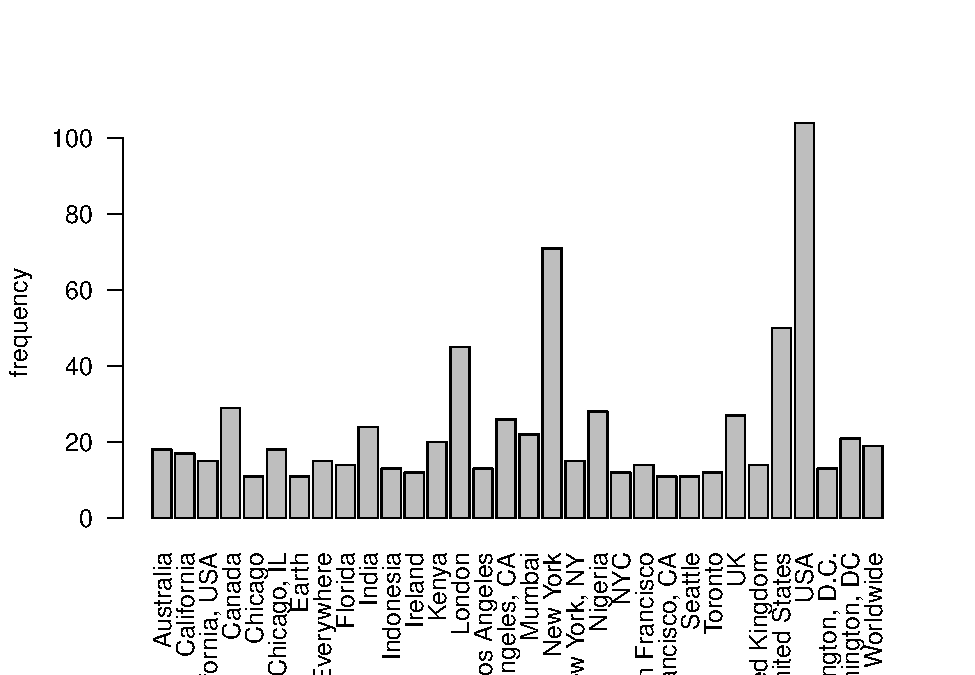
\includegraphics[width=0.8\linewidth]{document_files/figure-latex/unnamed-chunk-9-1} 
		\caption{ubicaciones que se repiten más de 10 veces.}
		\label{fig: ubicaciones que se repiten más de 10 veces}
	\end{center}
\end{figure}

El argumento \textbf{las} de la función \textbf{barplot} se usa para poner horizontalmente los nombres de las ubicaciones en el \textit{eje-x} de la Figura \ref{fig: ubicaciones que se repiten más de 10 veces}.

Del total de ubicaciones, 3342, la mayoría de ellas cuenta con menos de 10 observaciones. Teniendo en cuenta el análisis exploratorio de la variable \textbf{location} y acorde a nuestro criterio, no se considera buena para hacer predicciones, ya que la variable consta de muy pocas observaciones dentro del conjunto de datos (no es representativa), y puede ocurrir que, durante la realización de la validación cruzada o \emph{bootstrapping}, algunas de las muestras no contengan ninguna observación de dicha variable, lo que puede dar lugar a errores.

\begin{tcolorbox}
	Una muestra \emph{bootstrap} es una muestra obtenida a partir de la
	muestra original por muestreo aleatorio con reposición, y del mismo
	tamaño que la muestra original. Muestreo aleatorio con reposición
	(resampling with replacement) significa que, después de que una
	observación sea extraída, se vuelve a poner a disposición para las
	siguientes extracciones. Como resultado de este tipo de muestreo,
	algunas observaciones aparecerán múltiples veces en la muestra \emph{bootstrap} 
	y en otras ninguna.
\end{tcolorbox}

La variable \textbf{location} también la excluiremos en el \ref{preprocesado-de-los-datos}{procesamiento de texto}.

\hypertarget{variable-id}{%
\subsection{\texorpdfstring{Variable
\emph{id}}{Variable id}}\label{variable-id}}

La variable \textbf{id} es solo un identificador único, así que, no la
analizaremos y procederemos a eliminarla de los conjuntos de datos de
train y test.

\vspace{3mm}

\begin{Shaded}
\begin{Highlighting}[]
\NormalTok{train}\OperatorTok{$}\NormalTok{id <-}\StringTok{ }\OtherTok{NULL}
\NormalTok{test}\OperatorTok{$}\NormalTok{id <-}\StringTok{ }\OtherTok{NULL}
\end{Highlighting}
\end{Shaded}

\hypertarget{conclusiuxf3n-anuxe1lisis-exploratorio}{%
\subsection{Conclusión análisis
exploratorio}\label{conclusiuxf3n-anuxe1lisis-exploratorio}}

Llegados a este punto, después de un análisis exploratorio de las variables explicativas \textbf{keyword}, \textbf{location} y \textbf{id}, y el estudio de la distribución de la variable a predecir con sus posibles relaciones con estas variables, nuestro criterio es descartar-las para las futuras predicciones y el \ref{preprocesado-de-los-datos}{procesamiento de texto}. Consecuentemente nos centraremos en la variable \textbf{text} en la siguiente sección.

\hypertarget{procesamiento-de-texto}{%
\section{Procesamiento de texto}\label{procesamiento-de-texto}}

Combinamos los conjuntos de datos de train y test para ahorrar esfuerzos
en el \ref{preprocesado-de-los-datos}{preprocesado de datos}. Para ello, usamos la función
\textbf{bind\_rows()} del paquete \textbf{dplyr}, que nos permitirá enlazar de forma eficiente los dos
conjuntos de datos por fila y columna. Podremos comprobar que la
combinación se hace correctamente, sumando los elementos del conjunto de datos de train (7613)
y los elementos del conjunto de datos de test (3263), el nuevo conjunto de datos (\textbf{complete\_df})
tendrá 10876 observaciones, 3 variables explicativas (\textbf{keyword},
\textbf{location}, \textbf{text}) y la variable de clase
\textbf{target}.

\vspace{3mm}

\begin{Shaded}
\begin{Highlighting}[]
\NormalTok{complete_df <-}\StringTok{ }\KeywordTok{bind_rows}\NormalTok{(train, test)}
\KeywordTok{str}\NormalTok{(complete_df, }\DataTypeTok{width =} \DecValTok{85}\NormalTok{, }\DataTypeTok{strict.width =} \StringTok{"cut"}\NormalTok{)}
\end{Highlighting}
\end{Shaded}

\begin{verbatim}
## 'data.frame':    10876 obs. of  4 variables:
##  $ keyword : chr  NA NA NA NA ...
##  $ location: chr  NA NA NA NA ...
##  $ text    : chr  "Our Deeds are the Reason of this #earthquake May ALLAH Forgive "..
##  $ target  : Factor w/ 2 levels "No","Yes": 2 2 2 2 2 2 2 2 2 2 ...
\end{verbatim}

El \ref{preprocesado-de-los-datos}{preprocesado de datos} englobará las transformaciones de los textos de la variable \textbf{text}, como, por ejemplo la imputación de los valores ausentes o la reducción de
dimensionalidad del conjunto de datos \textbf{complete\_df}.

Ahora, vamos a mirar cuantos valores perdidos contiene nuestro conjunto de
datos \textbf{complete\_df}. La función \textbf{colSums()} sumará los
valores que la función \textbf{sapply()} del paquete \textbf{base} encuentre, en este caso, los
valores perdidos.

\vspace{3mm}

\begin{Shaded}
\begin{Highlighting}[]
\KeywordTok{colSums}\NormalTok{(}\KeywordTok{sapply}\NormalTok{(complete_df, is.na))}
\end{Highlighting}
\end{Shaded}

\begin{verbatim}
##  keyword location     text   target 
##       87     3638        0     3263
\end{verbatim}

Identificamos que las variables explicativas \textbf{keyword} y
\textbf{location} contienen valores perdidos. La variable explicativa
\textbf{text} no contienen valores perdidos. Sobretodo hay una gran cantidad
de tweets para los cuales falta su ubicación. Los 3263 valores perdidos
de la variable a predecir provienen del conjunto de datos de test. 

Nos ocuparemos de los valores perdidos más adelante.

\hypertarget{corpus}{%
\subsection{Corpus}\label{corpus}}

\begin{tcolorbox}
	Un corpus lingüístico se define como ``un conjunto de textos de un
	mismo origen'' y que tiene por función recopilar conjuntos de textos.
	El uso de un corpus lingüístico nos permitirá obtener información de las
	palabras utilizadas con más o menor frecuencia dentro del conjunto de datos.
\end{tcolorbox}

Con el nuevo conjunto de datos, \textbf{complete\_df},
procedemos a crear nuestro Corpus, es decir, un conjunto de textos a partir de los textos de la
variable \textbf{text}. El Corpus que se
compondrá de todos los textos de los tweets, lo asignaremos al objeto
\emph{myCorpus} usando las funciones \textbf{VectorSource()} y
\textbf{Corpus()}. La función \textbf{Corpus()} creará el Corpus a partir de un vector de textos que contiene los textos de todos los tweets. La función \textbf{VectorSource()} interpretará cada
mensaje de texto de los tweets como un elemento de ese vector de textos.

\begin{Shaded}
\begin{Highlighting}[]
\NormalTok{myCorpus <-}\StringTok{ }\KeywordTok{Corpus}\NormalTok{(}\KeywordTok{VectorSource}\NormalTok{(complete_df}\OperatorTok{$}\NormalTok{text))}
\NormalTok{myCorpus}
\end{Highlighting}
\end{Shaded}

\begin{verbatim}
## <<SimpleCorpus>>
## Metadata:  corpus specific: 1, document level (indexed): 0
## Content:  documents: 10876
\end{verbatim}

Nuestro Corpus está compuesto por 10876 conjuntos de textos.

\hypertarget{limpieza-del-texto}{%
\subsection{Limpieza del texto}\label{limpieza-del-texto}}

Como tenemos 10876 conjuntos de textos, necesitamos limpiarlos de caracteres que son de poca
utilidad. Eso nos ayudará a reducir su dimensionalidad. Para ello, mayoritariamente usaremos las funciones \textbf{gsub()} y \textbf{tm\_map()} del paquete \textbf{tm}. La función \textbf{gsub()} buscará y reemplazará desde la primera hasta la última de las coincidencias de un patrón (representado por una \emph{regular expression}). La función \textbf{tm\_map()} será la encargada de aplicar las diferentes transformaciones en los conjuntos de textos.

\begin{tcolorbox}
	Una expresión regular (o en inglés \emph{regular expression}) es una
	representación, según unas reglas sintácticas de un lenguaje formal, de
	una porción de texto genérico a buscar dentro de otro texto, como por
	ejemplo caracteres, palabras o patrones de texto concretos.
\end{tcolorbox}

Empezamos la limpieza eliminando los enlaces.

\begin{Shaded}
\begin{Highlighting}[]
\NormalTok{removeURL <-}\StringTok{ }\ControlFlowTok{function}\NormalTok{(x) }\KeywordTok{gsub}\NormalTok{(}\StringTok{"http[^[:space:]]*"}\NormalTok{, }\StringTok{""}\NormalTok{, x)  }
\NormalTok{myCorpus <-}\StringTok{ }\KeywordTok{tm_map}\NormalTok{(myCorpus, }\KeywordTok{content_transformer}\NormalTok{(removeURL))}
\end{Highlighting}
\end{Shaded}

Convertimos todo a minúsculas.

\begin{Shaded}
\begin{Highlighting}[]
\NormalTok{myCorpus <-}\StringTok{ }\KeywordTok{tm_map}\NormalTok{(myCorpus, }\KeywordTok{content_transformer}\NormalTok{(tolower))}
\end{Highlighting}
\end{Shaded}

Eliminamos los nombres de usuario.

\begin{Shaded}
\begin{Highlighting}[]
\NormalTok{removeUsername <-}\StringTok{ }\ControlFlowTok{function}\NormalTok{(x) }\KeywordTok{gsub}\NormalTok{(}\StringTok{"@[^[:space:]]*"}\NormalTok{, }\StringTok{""}\NormalTok{, x)  }
\NormalTok{myCorpus <-}\StringTok{ }\KeywordTok{tm_map}\NormalTok{(myCorpus, }\KeywordTok{content_transformer}\NormalTok{(removeUsername))}
\end{Highlighting}
\end{Shaded}

Nos deshacemos de la puntuación, puesto que por ejemplo ``fin'' y
``fin.'' son identificadas como palabras diferentes, lo cual no
deseamos.

\begin{Shaded}
\begin{Highlighting}[]
\NormalTok{removeNumPunct <-}\StringTok{ }\ControlFlowTok{function}\NormalTok{(x) }\KeywordTok{gsub}\NormalTok{(}\StringTok{"[^[:alpha:][:space:]]*"}\NormalTok{, }\StringTok{""}\NormalTok{, x)   }
\NormalTok{myCorpus <-}\StringTok{ }\KeywordTok{tm_map}\NormalTok{(myCorpus, }\KeywordTok{content_transformer}\NormalTok{(removeNumPunct))}
\end{Highlighting}
\end{Shaded}

Usamos la función \textbf{stopwords(``english'')},
recordemos que los textos de los tweets están en inglés, y cada idioma
tiene sus propias palabras vacías; para eliminar las palabras vacías, es
decir, aquellas que consideramos que tienen poco valor de análisis para nuestro ejercicio, que carecen de un
significado por si solas, tales como artículos, preposiciones,
conjunciones, pronombres, etc.

\begin{Shaded}
\begin{Highlighting}[]
\NormalTok{myStopWords <-}\StringTok{ }\KeywordTok{c}\NormalTok{((}\KeywordTok{stopwords}\NormalTok{(}\StringTok{'english'}\NormalTok{)), }
    \KeywordTok{c}\NormalTok{(}\StringTok{"really"}\NormalTok{, }\StringTok{"tweets"}\NormalTok{, }\StringTok{"saw"}\NormalTok{, }\StringTok{"just"}\NormalTok{, }\StringTok{"feel"}\NormalTok{, }\StringTok{"may"}\NormalTok{, }\StringTok{"us"}\NormalTok{, }\StringTok{"rt"}\NormalTok{, }\StringTok{"every"}\NormalTok{, }\StringTok{"one"}\NormalTok{,}
     \StringTok{"amp"}\NormalTok{, }\StringTok{"like"}\NormalTok{, }\StringTok{"will"}\NormalTok{, }\StringTok{"got"}\NormalTok{, }\StringTok{"new"}\NormalTok{, }\StringTok{"can"}\NormalTok{, }\StringTok{"still"}\NormalTok{, }\StringTok{"back"}\NormalTok{, }\StringTok{"top"}\NormalTok{, }\StringTok{"much"}\NormalTok{,}
     \StringTok{"near"}\NormalTok{, }\StringTok{"im"}\NormalTok{, }\StringTok{"see"}\NormalTok{, }\StringTok{"via"}\NormalTok{, }\StringTok{"get"}\NormalTok{, }\StringTok{"now"}\NormalTok{, }\StringTok{"come"}\NormalTok{, }\StringTok{"oil"}\NormalTok{, }\StringTok{"let"}\NormalTok{, }\StringTok{"god"}\NormalTok{, }\StringTok{"want"}\NormalTok{,}
     \StringTok{"pm"}\NormalTok{, }\StringTok{"last"}\NormalTok{, }\StringTok{"hope"}\NormalTok{, }\StringTok{"since"}\NormalTok{, }\StringTok{"everyone"}\NormalTok{, }\StringTok{"food"}\NormalTok{, }\StringTok{"content"}\NormalTok{, }\StringTok{"always"}\NormalTok{, }\StringTok{"th"}\NormalTok{,}
     \StringTok{"full"}\NormalTok{, }\StringTok{"found"}\NormalTok{, }\StringTok{"dont"}\NormalTok{, }\StringTok{"look"}\NormalTok{, }\StringTok{"cant"}\NormalTok{, }\StringTok{"mh"}\NormalTok{, }\StringTok{"lol"}\NormalTok{, }\StringTok{"set"}\NormalTok{, }\StringTok{"old"}\NormalTok{, }\StringTok{"service"}\NormalTok{,}
     \StringTok{"city"}\NormalTok{, }\StringTok{"home"}\NormalTok{, }\StringTok{"live"}\NormalTok{, }\StringTok{"night"}\NormalTok{, }\StringTok{"news"}\NormalTok{, }\StringTok{"say"}\NormalTok{, }\StringTok{"video"}\NormalTok{, }\StringTok{"people"}\NormalTok{, }\StringTok{"ill"}\NormalTok{, }
     \StringTok{"way"}\NormalTok{,  }\StringTok{"please"}\NormalTok{, }\StringTok{"years"}\NormalTok{, }\StringTok{"take"}\NormalTok{, }\StringTok{"homes"}\NormalTok{, }\StringTok{"read"}\NormalTok{, }\StringTok{"man"}\NormalTok{, }\StringTok{"next"}\NormalTok{, }\StringTok{"cross"}\NormalTok{, }
     \StringTok{"boy"}\NormalTok{, }\StringTok{"bad"}\NormalTok{, }\StringTok{"ass"}\NormalTok{))}

\KeywordTok{head}\NormalTok{(myStopWords, }\DecValTok{30}\NormalTok{)}
\end{Highlighting}
\end{Shaded}

\begin{verbatim}
##  [1] "i"          "me"         "my"         "myself"     "we"        
##  [6] "our"        "ours"       "ourselves"  "you"        "your"      
## [11] "yours"      "yourself"   "yourselves" "he"         "him"       
## [16] "his"        "himself"    "she"        "her"        "hers"      
## [21] "herself"    "it"         "its"        "itself"     "they"      
## [26] "them"       "their"      "theirs"     "themselves" "what"
\end{verbatim}

\begin{Shaded}
\begin{Highlighting}[]
\NormalTok{myCorpus <-}\StringTok{ }\KeywordTok{tm_map}\NormalTok{(myCorpus, removeWords, myStopWords) }
\end{Highlighting}
\end{Shaded}

Podemos observar que se han añadido (de manera aleatoria) algunas palabras vacías de más como: ``really'', ``tweets'' y ``saw''. Porqué son de las más usadas en los mensajes de texto de los tweets en Twitter (ver el siguiente \href{https://techland.time.com/2009/06/08/the-500-most-frequently-used-words-on-twitter/}{\color{blue}enlace} para ver las 500 palabras más usadas en esta red social). Si son palabras muy utilizadas contendrán poco valor de análisis para nuestro ejercicio.

Eliminamos las palabras de una sola letra.

\begin{Shaded}
\begin{Highlighting}[]
\NormalTok{removeSingle <-}\StringTok{ }\ControlFlowTok{function}\NormalTok{(x) }\KeywordTok{gsub}\NormalTok{(}\StringTok{" . "}\NormalTok{, }\StringTok{" "}\NormalTok{, x)   }
\NormalTok{myCorpus <-}\StringTok{ }\KeywordTok{tm_map}\NormalTok{(myCorpus, }\KeywordTok{content_transformer}\NormalTok{(removeSingle))}
\end{Highlighting}
\end{Shaded}

Por último, eliminamos los espacios vacíos excesivos. Muchos de ellos son
introducidos por las transformaciones anteriores.

\begin{Shaded}
\begin{Highlighting}[]
\NormalTok{myCorpus <-}\StringTok{ }\KeywordTok{tm_map}\NormalTok{(myCorpus, }\KeywordTok{content_transformer}\NormalTok{(stripWhitespace))}
\end{Highlighting}
\end{Shaded}

La limpieza del texto, és un proceso básico dentro del Procesamiento del Lenguaje Natural (PLN), que reduce de manera significativa la longitud del conjunto de textos del Corpus. 

\hypertarget{creaciuxf3n-de-un-modelo-predictivo}{%
\section{Creación de un modelo
predictivo}\label{creaciuxf3n-de-un-modelo-predictivo}}

Para la creación de un modelo predictivo necesitamos construir una \textbf{Term Document Matrix} del conjunto de textos de nuestro Corpus, donde cada fila representará un texto y cada palabra (única) de un texto estará representada por una columna. Con esta matriz podremos empezar el preprocesado de datos y crear nuestro modelo predictivo más adelante.

\begin{tcolorbox}
	Una \textbf{Term Document Matrix} es una matriz matemática que describe la
	frecuencia con la que se repiten una serie de palabras en una colección
	de textos.
\end{tcolorbox}

\hypertarget{preprocesado-de-los-datos}{%
\subsection{Preprocesado de los datos}\label{preprocesado-de-los-datos}}

Sabemos que el preprocesado de datos engloba aquellas transformaciones de los datos con la finalidad de mejorar los resultados de la clasificación supervisada. Todo preprocesado de datos debe
aprenderse de las observaciones del conjunto de datos de train y luego aplicarse a los conjuntos de datos de train y de test. Esto es muy importante para no violar la condición
de que ninguna información procedente de las observaciones del conjunto de datos de test
influya en el ajuste del modelo predictivo.

Comenzaremos mapeando nuestro Corpus, indicando que es una Term
Document Matrix. Para ello, utilizamos la función \textbf{TermDocumentMatrix()} del paquete \textbf{tm} y
asignaremos el resultado al objeto \textbf{complete.tdm}. 

Con el argumento \textbf{control} de la función \textbf{TermDocumentMatrix()}, indicamos que evaluamos y incluimos todos los textos que tengan una longitud superior a 4 caracteres hasta \emph{Inf}, donde \emph{Inf} es el valor Infinito. De esta manera, conseguimos incluir la mayoría de los textos  del Corpus en la Term Document Matrix. Por defecto la función \textbf{TermDocumentMatrix()} usa el valor numérico \emph{tf-id}, que mide la importancia relativa de cada palabra de los textos, es decir, mide su frecuencia de ocurrencia. El valor \emph{tf-id} aumenta según el número de veces que una palabra aparece en un texto y no en otros, lo que permite averiguar qué palabras son más comunes en este texto respecto a los otros.

\begin{Shaded}
\begin{Highlighting}[]
\NormalTok{complete.tdm <-}\StringTok{ }\KeywordTok{TermDocumentMatrix}\NormalTok{(myCorpus, }\DataTypeTok{control=}\KeywordTok{list}\NormalTok{(}\DataTypeTok{wordLengths=} \KeywordTok{c}\NormalTok{(}\DecValTok{4}\NormalTok{, }\OtherTok{Inf}\NormalTok{)))}
\NormalTok{complete.tdm}
\end{Highlighting}
\end{Shaded}

\begin{verbatim}
## <<TermDocumentMatrix (terms: 16880, documents: 10876)>>
## Non-/sparse entries: 76219/183510661
## Sparsity           : 100%
## Maximal term length: 49
## Weighting          : term frequency (tf)
\end{verbatim}

Podemos observar que tenemos 16880 \emph{terms} en 10876 textos, esto quiere decir que
tenemos 16880 palabras diferentes en 10876 textos. Lo cual es una
cantidad considerable de palabras de la Term Document Matrix, pero no esperaríamos otra cosa de
una red social como Twitter. La palabra más larga contiene 49 caracteres.

Por ese motivo, usaremos la función \textbf{removeSparseItems()} del paquete \textbf{tm} para depurar nuestra
Term Document Matrix de aquellas palabras que aparecen con muy poca frecuencia, es decir, que son dispersas. Con demasiadas palabras seria posible que no podamos entrenar nuestro modelo debido a grandes restricciones computacionales.

La función \textbf{removeSparseItems()} requiere que especifiquemos el argumento \textbf{sparse}, que puede asumir valores de 0 a 1. Este valor representa la dispersión de las palabras que queremos conservar. Si lo fijamos muy alto (cerca de 1, pero no 1), conservaremos muchas palabras, casi todas, pues estamos
indicando que queremos conservar palabras, aunque sean muy dispersas. Naturalmente, ocurre lo opuesto si fijamos este valor muy bajo (cerca de 0, pero no 0), pudiendo incluso quedarnos sin ninguna palabra, si las palabras en nuestros textos son bastante dispersas en general.

Para nuestro ejercicio, se decide fijar el valor del argumento \textbf{sparse} a \emph{.9975}, con la intención de conservar las palabras que aparecen al menos en el 0.25\% de las observaciones. Lo vemos a continuación.

\vspace{3mm}

\begin{Shaded}
\begin{Highlighting}[]
\NormalTok{complete.tdm <-}\StringTok{ }\KeywordTok{removeSparseTerms}\NormalTok{(complete.tdm, }\DataTypeTok{sparse =} \FloatTok{.9975}\NormalTok{)}
\NormalTok{complete.tdm}
\end{Highlighting}
\end{Shaded}

\begin{verbatim}
## <<TermDocumentMatrix (terms: 582, documents: 10876)>>
## Non-/sparse entries: 31214/6298618
## Sparsity           : 100%
## Maximal term length: 17
## Weighting          : term frequency (tf)
\end{verbatim}

De las 16880 palabras que teníamos, nos hemos quedado con 582, lo cual
reduce en gran medida la dificultad y complejidad del problema de
\emph{alta dimensionalidad}, lo cual es muy deseable. La palabra más larga ahora
contiene 17 caracteres.

\hypertarget{feature-extraction-mediante-singular-value-decomposition}{%
\subsubsection{Feature Extraction mediante SVD}\label{feature-extraction-mediante-singular-value-decomposition}}

La descomposición de los datos originales en un nuevo conjunto de datos, sin
necesidad de pérdida de información relevante y sacando a la luz la
información existente, es un proceso de vital importancia para implementar
la parte más computacionalmente intensa correspondiente a la \href{https://es.wikipedia.org/wiki/Miner\%C3\%ADa_de_textos}{\color{blue}minería de textos} del ejercicio. 

Buscando una intuitiva separabilidad de las clases de los datos aplicaremos la
técnica denominada como \emph{Descomposición en Valores Singulares (SVD)}, en nuestra Term Document Matrix.

\begin{tcolorbox}
	La \href{https://es.wikipedia.org/wiki/Descomposici\%C3\%B3n_en_valores_singulares}{\color{blue}Descomposición de Valores Singulares} (en inglés Singular Value Decomposition (SVD) es una técnica de reducción de la dimensionalidad en minería de textos, que puede utilizarse para descubrir las dimensiones existentes que determinan similitudes semánticas entre las palabras (unidades léxicas) o entre los textos (unidades de	contexto).
\end{tcolorbox}

Para aplicar la técnica denominada como \emph{Descomposición en Valores Singulares
(SVD)} tenemos que transformar nuestra Term Document Matrix en una \href{https://es.wikipedia.org/wiki/Matriz_transpuesta}{\color{blue}matriz transpuesta} que llamaremos \textbf{complete.term.matrix} para la factorización de la misma. 

Para crear la matriz transpuesta usamos la función \textbf{t()} del paquete \textbf{base} y la convertimos en un objeto de tipo \textbf{matrix}. Nos aseguraremos que la matriz transpuesta no contiene valores perdidos, usando la función \textbf{which()}.

\begin{Shaded}
\begin{Highlighting}[]
\NormalTok{complete.term.matrix <-}\StringTok{ }\KeywordTok{as.matrix}\NormalTok{(t(complete.tdm))}
\KeywordTok{which}\NormalTok{(!complete.cases(complete.term.matrix))}
\end{Highlighting}
\end{Shaded}

\begin{verbatim}
## integer(0)
\end{verbatim}

La matriz transpuesta no contiene valores perdidos, podemos comenzar con la factorización de ésta. Para ello usaremos la función \textbf{irlba()}, que descompondrá la matriz transpuesta en los 150 vectores singulares más importantes, después de buscar un máximo de 600 iteraciones. El resultado se almacenará en el objeto \textbf{complete\_irlba}.

\begin{Shaded}
\begin{Highlighting}[]
\NormalTok{cl <-}\StringTok{ }\KeywordTok{makePSOCKcluster}\NormalTok{(}\DecValTok{4}\NormalTok{, }\DataTypeTok{setup_strategy=}\StringTok{"sequential"}\NormalTok{)}
\KeywordTok{registerDoParallel}\NormalTok{(cl)}

\NormalTok{complete_irlba <-}\StringTok{ }\KeywordTok{irlba}\NormalTok{(}\KeywordTok{t}\NormalTok{(complete.term.matrix), }\DataTypeTok{nv =} \DecValTok{150}\NormalTok{, }\DataTypeTok{maxit =} \DecValTok{600}\NormalTok{)}
\NormalTok{complete_irlba}\OperatorTok{$}\NormalTok{v[}\DecValTok{1}\OperatorTok{:}\DecValTok{10}\NormalTok{, }\DecValTok{1}\OperatorTok{:}\DecValTok{5}\NormalTok{]}
\end{Highlighting}
\end{Shaded}

\begin{verbatim}
##                [,1]          [,2]          [,3]          [,4]          [,5]
##  [1,] -0.0003162281 -2.109638e-04 -3.318231e-04 -2.035137e-05  0.0008660149
##  [2,] -0.0431207327  1.408993e-02  5.124787e-03  3.922969e-03 -0.0021251369
##  [3,] -0.0020297768  2.205792e-04 -5.231801e-05  1.014223e-04  0.0008899277
##  [4,] -0.0054444920  1.259299e-04 -3.441743e-03  1.669137e-04  0.0094345444
##  [5,] -0.0021975777  8.533917e-05  7.910354e-05 -7.809264e-05  0.0017043646
##  [6,] -0.0449020384  1.303972e-02  1.677561e-03  3.883599e-03 -0.0005116573
##  [7,] -0.0060579030 -8.521515e-03 -3.239198e-02  6.490016e-04 -0.0023784289
##  [8,] -0.0387247287  1.297783e-02  5.140001e-03  3.764856e-03 -0.0112714576
##  [9,] -0.0079142623 -5.649745e-04 -6.691751e-04 -4.606357e-04  0.0135358450
## [10,] -0.0014005942 -2.762898e-04 -3.440679e-04 -4.573951e-05  0.0016280077
\end{verbatim}

\begin{Shaded}
\begin{Highlighting}[]
\KeywordTok{stopCluster}\NormalTok{(cl)}
\end{Highlighting}
\end{Shaded}

Lo que vemos arriba es una pequeña parte de la matriz transpuesta factorizada, que usaremos como
característica principal para la clasificación supervisada. Porqué con el rango de factorización, que indica las similitudes de las palabras en los textos, nos permitirá agrupar las palabras para su clasificación.

\hypertarget{divisiuxf3n-de-los-datos-en-train-y-test}{%
\subsection{División de los datos en train y
test}\label{divisiuxf3n-de-los-datos-en-train-y-test}}

Evaluar la capacidad predictiva de un modelo consiste en comprobar cómo
de próximas son sus predicciones a los verdaderos valores de la variable
a predecir. Para poder cuantificar lo de forma correcta, se
necesita disponer de un conjunto de observaciones, de las que se conozca
la variable a predecir, pero que el modelo no haya ``visto'', es decir,
que no hayan participado en su ajuste. Con esta finalidad, se dividen
los datos que tenemos en \textbf{complete\_df} en un conjunto de datos de 
train y un conjunto de datos de test.

Con el conjunto de datos, del que se conoce la variable a predecir (\textbf{complete\_df}) y la matriz transpuesta que hemos creado y factorizado en la sección anterior (\textbf{complete\_irlba}) creamos un nuevo objeto de tipo dataframe (\textbf{complete.svd}) que a continuación dividiremos en un conjunto de datos de train (\textbf{train.df}) y en un conjunto de datos de test (\textbf{test.df}), con el mismo tamaño de la partición inicial proporcionada por la competición de Kaggle que hemos elegido para nuestro ejercicio. En esta partición inicial el conjunto de datos de train cuenta con 7613
instancias y el conjunto de datos de test con 3263 instancias. Ver sección del \ref{anuxe1lisis-exploratorio-de-los-datos}{análisis exploratorio de los datos} para comprobarlo.

\begin{Shaded}
\begin{Highlighting}[]
\NormalTok{complete.svd <-}\StringTok{ }\KeywordTok{data.frame}\NormalTok{(}\DataTypeTok{target=}\NormalTok{complete_df}\OperatorTok{$}\NormalTok{target, complete_irlba}\OperatorTok{$}\NormalTok{v)}
\NormalTok{train.df <-}\StringTok{ }\NormalTok{complete.svd[}\DecValTok{1}\OperatorTok{:}\DecValTok{7613}\NormalTok{, ]}
\NormalTok{test.df <-}\StringTok{ }\NormalTok{complete.svd[}\DecValTok{7614}\OperatorTok{:}\DecValTok{10876}\NormalTok{, }\DecValTok{-1}\NormalTok{]}
\KeywordTok{dim}\NormalTok{(train.df)}
\end{Highlighting}
\end{Shaded}

\begin{verbatim}
## [1] 7613  151
\end{verbatim}

\begin{Shaded}
\begin{Highlighting}[]
\KeywordTok{dim}\NormalTok{(test.df)}
\end{Highlighting}
\end{Shaded}

\begin{verbatim}
## [1] 3263  150
\end{verbatim}

Vemos que usando la función \textbf{dim()}, los nuevos conjuntos de datos de train (\textbf{train.df}) y de test (\textbf{test.df}) tienen el mismo número de observaciones que la partición inicial.

Otra comprobación importante, es verificar que la distribución de la variable a predecir \textbf{target}, del nuevo conjunto datos de train \textbf{train.df}, no ha cambiado respecto a la partición inicial \textbf{complete\_df}. Si transformamos las variables \textbf{complete\_df\$target} y \textbf{train.df\$target} en un objeto de tipo \textbf{table} podremos usar la función \textbf{prop.table()} para ver las proporciones de cada clase y compararlas.

\vspace{2mm}

\begin{Shaded}
\begin{Highlighting}[]
\KeywordTok{prop.table}\NormalTok{(}\KeywordTok{table}\NormalTok{(complete_df}\OperatorTok{$}\NormalTok{target))}
\end{Highlighting}
\end{Shaded}

\begin{verbatim}
## 
##        No       Yes 
## 0.5703402 0.4296598
\end{verbatim}

\begin{Shaded}
\begin{Highlighting}[]
\KeywordTok{prop.table}\NormalTok{(}\KeywordTok{table}\NormalTok{(train.df}\OperatorTok{$}\NormalTok{target))}
\end{Highlighting}
\end{Shaded}

\begin{verbatim}
## 
##        No       Yes 
## 0.5703402 0.4296598
\end{verbatim}

La distribución de la variable a predecir no ha cambiado.

\hypertarget{selecciuxf3n-de-variables}{%
\subsection{Selección de variables}\label{selecciuxf3n-de-variables}}

Cuando se entrena un modelo de clasificación supervisada, es importante incluir como variables únicamente aquellas variables que están realmente relacionadas con la variable a predecir, ya que son estas las que contienen información útil para el modelo. Incluir un exceso de variables suele conllevar una reducción de la capacidad de predicción de los modelos. En este punto, es donde la selección de variables para puede suponer la diferencia entre un modelo normal y uno muy bueno.

\textbf{caret} posee una colección de herramientas internas para la selección de variables. Estas herramientas contienen sus propias estrategias de selección de variables. Por este motivo los modelos de \textbf{caret} como \textit{random forest, lasso o boosting} son tan versátiles.

Muchos de los modelos a los que se puede acceder mediante la función \textbf{train()} de \textbf{caret} producen ecuaciones de predicción que no necesariamente utilizan todas las variables, ya que, estos modelos tienen una selección de variables incorporada. El uso de estos modelos con selección de variables incorporada siempre será más eficiente que otras estrategias de selección de variables, como los métodos \textit{wrapper} y los métodos de filtrado.

Suponiendo que la selección de variables incorporada en los modelos de \textbf{caret} es la mejor para cada modelo, para este ejercicio escogemos y entrenaremos en la siguiente sección los siguientes algoritmos:

\begin{itemize}
	\item \textbf{glmnet}. Generalized Linear Model with Stepwise Feature Selection.
	\item \textbf{rf}. Random Forest.
	\item \textbf{gbm}. Stochastic Gradient Boosting.
\end{itemize}

Todos los algoritmos con selección de variables incorporada se encuentran disponibles en el siguiente \href{http://topepo.github.io/caret/feature-selection-overview.html}{\color{blue}enlace}.

Sabemos que hacer una buena selección de variables puede suponer la diferencia entre un modelo normal y uno muy bueno, pero ninguno de los algoritmos que se han seleccionado se utilizan específicamente en minería de textos. Así que, también entrenaremos el modelo \textbf{svmRadial} de \textbf{caret}. \textbf{svmRadial} es un algoritmo de clasificación supervisada utilizado en minería de textos. La finalidad de esta elección es poner de manifiesto que esto  también puede ser un elemento muy relevante para nuestro ejercicio.

Con el modelo \textbf{svmRadial} de \textbf{caret} no podemos incorporar la selección de variables usando la función \textbf{train()}. En este caso tendríamos que utilizar alguno de los métodos de selección de variables que nos ofrece \textbf{caret}, como el denominado \textit{recursive feature elimination} con la función \textbf{rfe()}, mediante un \textit{algoritmo genético} con la función \textbf{gafs.default()}, etc. Pero no utilizaremos ningún método de selección de variables, porqué queremos probar si \textbf{svmRadial} es mejor clasificador en comparación con los modelos que sí incorporan la selección de variables mediante la función \textbf{train()}. 

\begin{tcolorbox}
	Más información sobre las funciones de \textbf{caret} \textbf{rfe()} i \textbf{gafs.default()}:
	\begin{itemize}
		\item \url{https://www.rdocumentation.org/packages/caret/versions/6.0-86/topics/rfe} 
		\item \url{https://www.rdocumentation.org/packages/caret/versions/6.0-86/topics/gafs.default}
	\end{itemize}
\end{tcolorbox}

\hypertarget{entrenamiento-de-modelos}{%
\subsection{Entrenamiento de modelos}\label{entrenamiento-de-modelos}}

En esta sección se entrenan los diferentes modelos elegidos de clasificación
supervisada con el objetivo de compararlos e identificar el que mejor
resultado obtiene prediciendo. Todos estos modelos incorporados en el
paquete \textbf{caret} se entrenan con la función \textbf{train()}. Entre
los argumentos de esta función destacan:

\begin{itemize}
\item
  \textbf{method}. El nombre del algoritmo que se desea emplear
  (\href{http://topepo.github.io/caret/available-models.html}{\color{blue}modelos disponibles}).
\item
  \textbf{metric}. La métrica que se usa para evaluar la capacidad
  predictiva del modelo. Aunque en la competición de Kaggle en la que se
  basa nuestro ejercicio se espera \textbf{F1} como métrica de
  evaluación, para cuantificar como de bueno son nuestros modelos
  utilizaremos la métrica de evaluación \textbf{Accuracy}. Porqué la
  distribución de la variable clase no presenta un problema notable de
  desbalanceo de clases y cuando la distribución de la variable clase
  está bastante equilibrada se considera una buena medida de evaluación.
\end{itemize}

\begin{tcolorbox}
	La métrica de evaluación \textbf{Accuracy} representa el porcentaje de observaciones correctamente
	clasificadas respecto al total de predicciones.
\end{tcolorbox}

\begin{itemize}
\tightlist
\item
  \textbf{trControl}. Especificaciones adicionales sobre la forma de
  llevar a cabo el entrenamiento del modelo.
\end{itemize}

Para especificar el tipo de validación que se usará durante el entrenamiento, se crea un control de entrenamiento mediante la función \textbf{trainControl()}, donde se pasa al argumento \textbf{trControl} de la función \textbf{train()}. Para nuestro ejercicio, el tipo de validación que se desarrolla es una \textbf{repeated K-Fold Cross-Validation}. 

Con la función \textbf{createMultiFolds()} repartimos las observaciones del conjunto de datos de train en 5 folds (conjuntos) del mismo tamaño (\emph{k=5}), y los repetiremos 3 veces (\emph{times=3}). En total tendremos 5 * 3 = 15 folds en el objeto \textbf{cv.folds}.

Veremos que durante el entrenamiento de los modelos se usan semillas con \textbf{set.seed(123)}. Las semillas son necesarias si se quiere asegurar la reproducibilidad de los resultados finales, ya que la validación cruzada implican selección aleatoria.

\vspace{3mm}

\begin{Shaded}
\begin{Highlighting}[]
\KeywordTok{set.seed}\NormalTok{(}\DecValTok{123}\NormalTok{)}
\NormalTok{cv.folds <-}\StringTok{ }\KeywordTok{createMultiFolds}\NormalTok{(train.df}\OperatorTok{$}\NormalTok{target, }\DataTypeTok{k=}\DecValTok{5}\NormalTok{, }\DataTypeTok{times=}\DecValTok{3}\NormalTok{)}
\NormalTok{cv.cntrl <-}\StringTok{ }\KeywordTok{trainControl}\NormalTok{(}\DataTypeTok{method=}\StringTok{"repeatecv"}\NormalTok{, }\DataTypeTok{number=}\DecValTok{5}\NormalTok{,}
                         \DataTypeTok{index=}\NormalTok{cv.folds, }\DataTypeTok{allowParallel=}\OtherTok{TRUE}\NormalTok{, }
                         \DataTypeTok{returnResamp=}\StringTok{"final"}\NormalTok{,}
                         \DataTypeTok{verboseIter=}\OtherTok{FALSE}\NormalTok{)}
\end{Highlighting}
\end{Shaded}

El argumento \textbf{method} de la función \textbf{trainControl()} hace
posible utilizar distintos tipos de validación. La \textbf{repeated K-Fold Cross-Validation} se denomina
``repeatecv''. Además de fijar el tipo de validación, la función \textbf{trainControl()} permite
fijar multitud de argumentos. 

A continuación, describimos los argumentos que se han fijado:

\begin{itemize}
\tightlist
\item
  \textbf{number}. El número de folds. 
  
  Tiene que coincidir con el argumento \textit{k} de la función \textbf{createMultiFolds()}. 
\item
  \textbf{index}. Lista de los elementos de (\textbf{cv.folds}). Cada elemento de la lista es un vector que contiene el fold correspondiente a cada repetición. 
\end{itemize}

\vspace{2mm}

\begin{Shaded}
\begin{Highlighting}[]
\KeywordTok{str}\NormalTok{(cv.folds)}
\end{Highlighting}
\end{Shaded}

\begin{verbatim}
## List of 15
##  $ Fold1.Rep1: int [1:6090] 1 2 3 4 5 6 7 8 9 11 ...
##  $ Fold2.Rep1: int [1:6090] 1 2 3 4 5 7 8 9 10 11 ...
##  $ Fold3.Rep1: int [1:6090] 1 2 3 5 6 7 8 9 10 11 ...
##  $ Fold4.Rep1: int [1:6091] 2 3 4 6 10 12 13 14 15 16 ...
##  $ Fold5.Rep1: int [1:6091] 1 4 5 6 7 8 9 10 11 12 ...
##  $ Fold1.Rep2: int [1:6090] 1 4 5 6 8 9 10 11 12 13 ...
##  $ Fold2.Rep2: int [1:6090] 2 3 4 5 6 7 8 9 11 12 ...
##  $ Fold3.Rep2: int [1:6090] 1 2 3 5 6 7 10 11 12 14 ...
##  $ Fold4.Rep2: int [1:6091] 1 2 3 4 5 6 7 8 9 10 ...
##  $ Fold5.Rep2: int [1:6091] 1 2 3 4 7 8 9 10 11 12 ...
##  $ Fold1.Rep3: int [1:6091] 1 2 3 6 7 8 9 10 11 12 ...
##  $ Fold2.Rep3: int [1:6090] 1 2 4 5 6 7 9 10 11 13 ...
##  $ Fold3.Rep3: int [1:6090] 1 3 4 5 8 9 10 11 12 13 ...
##  $ Fold4.Rep3: int [1:6090] 2 3 4 5 6 7 8 12 13 14 ...
##  $ Fold5.Rep3: int [1:6091] 1 2 3 4 5 6 7 8 9 10 ...
\end{verbatim}

\vspace{2mm}

\begin{itemize}
\tightlist
\item
  \textbf{allowParallel}. Habilita la computación paralela. 

\item
  \textbf{returnResamp}. Indica la cantidad de métricas de evaluación que se deben guardar por cada repetición. Se especifica que se almacene la información ``final'' de los modelos generados en todas las repeticiones. 
  
\item
  \textbf{verboseIter}. Para mostrar o no el registro del entrenamiento. En nuestro caso no se mostrará.
\end{itemize}

Muchos modelos contienen parámetros que no pueden aprenderse a partir de
los datos de entrenamiento y por lo tanto, deben de ser establecidos
por nosotros. A estos se les conoce como \emph{hiperparámetros},
argumento \textbf{tunning} de \textbf{caret}. Con la función
\textbf{expand.grid()} definiremos los valores de los parámetros a tunear.

Los resultados de un modelo pueden depender en gran medida del valor que
tomen estos \emph{hiperparámetros}, sin embargo, no se pueden conocer de
antemano cuáles son los más adecuados. La forma más común de encontrarlos 
es probando diferentes posibilidades. Para ello se
utiliza el argumento de \textbf{caret} \textbf{tuneGrid} como argumento de la función
\textbf{train()}. Si no se tiene ninguna idea de qué 
\emph{hiperparámetros} pueden ser los más adecuados, lo mejor es utilizar la
aleatoriedad. \textbf{caret} también incorpora esta opción mediante el
argumento \textbf{tuneLength}, también se lo pasamos a la función
\textbf{train()}.

Durante el entrenamiento de los modelos usaremos \textbf{tuneGrid} 
y \textbf{tuneLength} según nuestro criterio. El uso de \textbf{tuneGrid} será mayor, ya
que, de esta forma, se evita que se generen automáticamente valores que
no tienen sentido o que disparan el tiempo de computación necesario.

\begin{tcolorbox}
	\textbf{k-Fold-Cross-Validation}. Las observaciones de entrenamiento
	se reparten en k folds (conjuntos) del mismo tamaño. El modelo se ajusta
	con todas las observaciones excepto las del primer fold y se evalúa
	prediciendo las observaciones del fold que ha quedado excluido,
	obteniendo así la primera métrica. El proceso se repite k veces,
	excluyendo un fold distinto en cada iteración. Al final, se generan k
	valores de la métrica, que se agregan (normalmente con la media y la
	desviación típica) generando la estimación final de validación.	
\end{tcolorbox}

\begin{tcolorbox}
	\textbf{repeated k-Fold-Cross-Validation}. Es exactamente
	igual al método k-Fold-Cross-Validation pero repitiendo el proceso
	completo n veces. Por ejemplo, 10-Fold-Cross-Validation con 5
	repeticiones implica a un total de 50 iteraciones,
	pero no equivale a un 50-Fold-Cross-Validation.
\end{tcolorbox}

A lo largo del proceso de entrenamiento de los modelos es donde más destacarán las
funcionalidades ofrecidas por \textbf{caret}, permitiendo emplear la
misma sintaxis para ajustar, optimizar, evaluar y predecir un amplio
abanico de modelos variando únicamente el nombre del algoritmo. Aunque
\textbf{caret} permite todo esto con apenas unas pocas líneas de código
son muchos los argumentos que pueden ser adaptados, cada uno con
múltiples posibilidades. Con el objetivo de exponer mejor cada una de
las opciones, en lugar de crear directamente un modelo final, se
entrenaran los modelos que hemos seleccionado en la sección de 
\ref{selecciuxf3n-de-variables}{selección de variables}.


\hypertarget{regresiuxf3n-loguxedstica}{%
\subsubsection{Regresión Logística}\label{regresiuxf3n-loguxedstica}}

Información detallada sobre regresión logística en
\href{https://www.cienciadedatos.net/documentos/27_regresion_logistica_simple_y_multiple}{\color{blue}Regresión
logística simple y múltiple}.

Entrenamos el modelo \textbf{glmnet} de \textbf{caret}. Este algoritmo no tiene
ningún \emph{hiperparámetro}, por lo tanto, usamos \textbf{tuneLength} igual a 15.

\vspace{3mm}

\begin{Shaded}
\begin{Highlighting}[]
\NormalTok{cl <-}\StringTok{ }\KeywordTok{makePSOCKcluster}\NormalTok{(}\DecValTok{6}\NormalTok{, }\DataTypeTok{setup_strategy=}\StringTok{"sequential"}\NormalTok{)}
\KeywordTok{registerDoParallel}\NormalTok{(cl)}
\end{Highlighting}
\end{Shaded}

\begin{Shaded}
\begin{Highlighting}[]
\KeywordTok{set.seed}\NormalTok{(}\DecValTok{123}\NormalTok{)}
\NormalTok{model_glmnet <-}\StringTok{ }\KeywordTok{train}\NormalTok{(target }\OperatorTok{~}\StringTok{ }\NormalTok{., }\DataTypeTok{data=}\NormalTok{train.df,}
                      \DataTypeTok{method=}\StringTok{"glmnet"}\NormalTok{,}
                      \DataTypeTok{metric=}\StringTok{"Accuracy"}\NormalTok{,}
                      \DataTypeTok{trControl=}\NormalTok{cv.cntrl,}
                      \DataTypeTok{tuneLenght=}\DecValTok{15}\NormalTok{)}
\NormalTok{model_glmnet}
\end{Highlighting}
\end{Shaded}

\begin{verbatim}
## glmnet 
## 
## 7613 samples
##  150 predictor
##    2 classes: 'No', 'Yes' 
## 
## No pre-processing
## Resampling: 
## Summary of sample sizes: 6090, 6090, 6090, 6091, 6091, 6090, ... 
## Resampling results across tuning parameters:
## 
##   alpha  lambda        Accuracy   Kappa    
##   0.10   0.0001850059  0.7648316  0.5085381
##   0.10   0.0018500586  0.7650941  0.5087571
##   0.10   0.0185005864  0.7635180  0.5023833
##   0.55   0.0001850059  0.7648316  0.5084863
##   0.55   0.0018500586  0.7650943  0.5081484
##   0.55   0.0185005864  0.7487187  0.4642323
##   1.00   0.0001850059  0.7649630  0.5087688
##   1.00   0.0018500586  0.7639123  0.5051295
##   1.00   0.0185005864  0.7211778  0.3970376
## 
## Accuracy was used to select the optimal model using the largest value.
## The final values used for the model were alpha = 0.55 and lambda = 0.001850059.
\end{verbatim}

\begin{Shaded}
\begin{Highlighting}[]
\KeywordTok{stopCluster}\NormalTok{(cl)}
\end{Highlighting}
\end{Shaded}

El valor de \emph{Accuracy} promedio estimado mediante validación cruzada
repetida es de 0.7648316, el modelo predice correctamente el 76.5\% de
las veces.

\hypertarget{random-forest}{%
\subsubsection{Random Forest}\label{random-forest}}

Información detallada sobre Random Forest en
\href{https://www.cienciadedatos.net/documentos/33_arboles_de_prediccion_bagging_random_forest_boosting}{\color{blue}Árboles
de predicción}.

Entrenamos el modelo \textbf{rf} de \textbf{caret}. Este algoritmo tiene un \textit{hiperparámetro}:

\begin{itemize}
\tightlist
\item
  \textbf{mtry}. Número de valores seleccionados aleatoriamente en cada
  árbol. En este caso hemos escogido: 3, 4, 5 y 7.
\end{itemize}

\vspace{3mm}

\begin{Shaded}
\begin{Highlighting}[]
\NormalTok{cl <-}\StringTok{ }\KeywordTok{makePSOCKcluster}\NormalTok{(}\DecValTok{6}\NormalTok{, }\DataTypeTok{setup_strategy=}\StringTok{"sequential"}\NormalTok{)}
\KeywordTok{registerDoParallel}\NormalTok{(cl)}
\end{Highlighting}
\end{Shaded}

\begin{Shaded}
\begin{Highlighting}[]
\KeywordTok{set.seed}\NormalTok{(}\DecValTok{123}\NormalTok{)}
\NormalTok{cv.grid <-}\StringTok{ }\KeywordTok{expand.grid}\NormalTok{(}\DataTypeTok{mtry=}\KeywordTok{c}\NormalTok{(}\DecValTok{3}\NormalTok{, }\DecValTok{4}\NormalTok{, }\DecValTok{5}\NormalTok{, }\DecValTok{7}\NormalTok{))}
\NormalTok{model_rf <-}\StringTok{ }\KeywordTok{train}\NormalTok{(target }\OperatorTok{~}\StringTok{ }\NormalTok{., }\DataTypeTok{data=}\NormalTok{train.df,}
                      \DataTypeTok{method=}\StringTok{"rf"}\NormalTok{,}
                      \DataTypeTok{metric=}\StringTok{"Accuracy"}\NormalTok{,}
                      \DataTypeTok{trControl=}\NormalTok{cv.cntrl,}
                      \DataTypeTok{tuneGrid=}\NormalTok{cv.grid)}
\NormalTok{model_rf}
\end{Highlighting}
\end{Shaded}

\begin{verbatim}
## Random Forest 
## 
## 7613 samples
##  150 predictor
##    2 classes: 'No', 'Yes' 
## 
## No pre-processing
## Resampling: 
## Summary of sample sizes: 6090, 6090, 6090, 6091, 6091, 6090, ... 
## Resampling results across tuning parameters:
## 
##   mtry  Accuracy   Kappa    
##   3     0.7618968  0.5068252
##   4     0.7623348  0.5078468
##   5     0.7608022  0.5051518
##   7     0.7587883  0.5010024
## 
## Accuracy was used to select the optimal model using the largest value.
## The final value used for the model was mtry = 4.
\end{verbatim}

\begin{Shaded}
\begin{Highlighting}[]
\KeywordTok{stopCluster}\NormalTok{(cl)}
\end{Highlighting}
\end{Shaded}

Empleando un modelo Random Forest con mtry = 4, se consigue un
valor de \emph{Accuracy} promedio de validación igual a 0.7623348, el modelo
predice correctamente el 76.2\% de las veces.

\newpage

\hypertarget{gradient-boosting}{%
\subsubsection{Gradient Boosting}\label{gradient-boosting}}

Información detallada sobre boosting
\href{https://www.cienciadedatos.net/documentos/33_arboles_de_prediccion_bagging_random_forest_boosting}{\color{blue}Árboles
de predicción}.

Entrenamos el modelo \textbf{gbm}. El modelo \textbf{gbm} de \textbf{caret} emplea el paquete \textbf{gbm} que tendremos que cargar antes de entrenar el modelo. Este
algoritmo tiene 4 \emph{hiperparámetros}:

\begin{itemize}
\item
  \textbf{n.trees}. Número de iteraciones del algoritmo de boosting.
  Cuanto mayor es este valor, más se reduce el error de entrenamiento pero mayor es el coste computacional.
\item
  \textbf{interaction.depth}. El número total de divisiones que tiene el
  árbol. Emplear árboles que tienen ente 1 y 6 nodos suele dar buenos
  resultados.
\item
  \textbf{shrinkage}. Controla la complejidad del modelo. Es
  preferible mejorar un modelo mediante muchos pasos pequeños que
  mediante unos pocos pasos muy grandes. Por esta razón, se emplea un valor de
  \textbf{shrinkage} tan pequeño como sea posible, teniendo en cuenta
  que, cuanto menor sea, mayor el número de iteraciones necesarias. 
\item
  \textbf{n.minobsinnode}. Número mínimo de observaciones que debe tener
  cada nodo del árbol para poder ser dividido. Al igual que
  \textbf{interaction.depth}, permite controlar la complejidad del modelo.
\end{itemize}

Además de los \emph{hiperparámetros}, este modelo nos permite controlar 
otros dos valores más a tener en cuenta. Estos valores son:

\begin{itemize}
\item
  \textbf{distribution}. Determina la función de coste (\emph{loss
  function}). Algunas de las más utilizadas son: \emph{gaussian
  (squared loss)} para regresión, \emph{bernoulli} para clasificaciones
  binarias, \emph{multinomial} para clasificaciones con más de dos clases y
  \emph{adaboost} también para clasificaciones binarias, ya que emplea la función
  exponencial del algoritmo original
  \href{https://en.wikipedia.org/wiki/AdaBoost}{\color{blue}AdaBoost}.
\item
  \textbf{bag.fraction} (subsampling fraction). Fracción de
  observaciones del conjunto de datos train seleccionadas de forma aleatoria.
  Si su valor es 1, se emplea el algoritmo de \emph{Gradient
  Boosting}, si es menor que 1, se emplea \emph{Stochastic Gradient
  Boosting}. Por defecto su valor es 0.5.
\end{itemize}

En este caso, solo añadimos de más el valor de \textbf{distribution}. Como nuestro
ejercicio se basa en un problema de clasificación binaria elegimos \emph{adaboost}.

\vspace{3mm}

\begin{Shaded}
\begin{Highlighting}[]
\KeywordTok{library}\NormalTok{(gbm)}
\end{Highlighting}
\end{Shaded}

\begin{Shaded}
\begin{Highlighting}[]
\NormalTok{cl <-}\StringTok{ }\KeywordTok{makePSOCKcluster}\NormalTok{(}\DecValTok{6}\NormalTok{, }\DataTypeTok{setup_strategy=}\StringTok{"sequential"}\NormalTok{)}
\KeywordTok{registerDoParallel}\NormalTok{(cl)}
\end{Highlighting}
\end{Shaded}

\begin{Shaded}
\begin{Highlighting}[]
\KeywordTok{set.seed}\NormalTok{(}\DecValTok{123}\NormalTok{)}
\NormalTok{cv.grid <-}\StringTok{ }\KeywordTok{expand.grid}\NormalTok{(}\DataTypeTok{interaction.depth=}\KeywordTok{c}\NormalTok{(}\DecValTok{1}\NormalTok{, }\DecValTok{2}\NormalTok{),}
                       \DataTypeTok{n.trees=}\DecValTok{100}\NormalTok{,}
                       \DataTypeTok{shrinkage=}\KeywordTok{c}\NormalTok{(}\FloatTok{0.001}\NormalTok{, }\FloatTok{0.01}\NormalTok{, }\FloatTok{0.1}\NormalTok{),}
                       \DataTypeTok{n.minobsinnode=}\KeywordTok{c}\NormalTok{(}\DecValTok{2}\NormalTok{, }\DecValTok{5}\NormalTok{, }\DecValTok{15}\NormalTok{))}

\NormalTok{model_gbm <-}\StringTok{ }\KeywordTok{train}\NormalTok{(target }\OperatorTok{~}\StringTok{ }\NormalTok{., }\DataTypeTok{data=}\NormalTok{train.df,}
                  \DataTypeTok{method=}\StringTok{"gbm"}\NormalTok{,}
                  \DataTypeTok{metric=}\StringTok{"Accuracy"}\NormalTok{,}
                  \DataTypeTok{trControl=}\NormalTok{cv.cntrl,}
                  \DataTypeTok{tuneGrid=}\NormalTok{cv.grid,}
                  \DataTypeTok{distribution=}\StringTok{"adaboost"}\NormalTok{,}
                  \DataTypeTok{verbose=}\OtherTok{FALSE}\NormalTok{)}
\NormalTok{model_gbm}
\end{Highlighting}
\end{Shaded}

\newpage

\begin{verbatim}
## Stochastic Gradient Boosting 
## 
## 7613 samples
##  150 predictor
##    2 classes: 'No', 'Yes' 
## 
## No pre-processing
## Resampling: 
## Summary of sample sizes: 6090, 6090, 6090, 6091, 6091, 6090, ... 
## Resampling results across tuning parameters:
## 
##   shrinkage  interaction.depth  n.minobsinnode  Accuracy   Kappa    
##   0.001      1                   2              0.5703402  0.0000000
##   0.001      1                   5              0.5703402  0.0000000
##   0.001      1                  15              0.5703402  0.0000000
##   0.001      2                   2              0.5703402  0.0000000
##   0.001      2                   5              0.5703402  0.0000000
##   0.001      2                  15              0.5703402  0.0000000
##   0.010      1                   2              0.6553692  0.2397333
##   0.010      1                   5              0.6548878  0.2383772
##   0.010      1                  15              0.6544059  0.2374328
##   0.010      2                   2              0.6946872  0.3400736
##   0.010      2                   5              0.6931547  0.3366365
##   0.010      2                  15              0.6932867  0.3367455
##   0.100      1                   2              0.7244616  0.4220042
##   0.100      1                   5              0.7230157  0.4197413
##   0.100      1                  15              0.7235418  0.4199881
##   0.100      2                   2              0.7446022  0.4675017
##   0.100      2                   5              0.7438146  0.4658317
##   0.100      2                  15              0.7421065  0.4621889
## 
## Tuning parameter 'n.trees' was held constant at a value of 100
## Accuracy was used to select the optimal model using the largest value.
## The final values used for the model were n.trees = 100, interaction.depth =
##  2, shrinkage = 0.1 and n.minobsinnode = 2.
\end{verbatim}

\begin{Shaded}
\begin{Highlighting}[]
\KeywordTok{stopCluster}\NormalTok{(cl)}
\end{Highlighting}
\end{Shaded}

Empleando un modelo Boosting con n.trees = 100, interaction.depth = 2,
shrinkage = 0.1 y n.minobsinnode = 2 se consigue un valor de \emph{Accuracy}
promedio de validación igual a 0.7446022, el modelo predice
correctamente el 74.4\% de las veces.

\hypertarget{svm}{%
\subsubsection{SVM}\label{svm}}

Información detallada sobre SVM en
\href{https://www.cienciadedatos.net/documentos/34_maquinas_de_vector_soporte_support_vector_machines}{\color{blue}Support Vector Machines}.

Entrenamos el modelo \textbf{svmRadial} de \textbf{caret}. Este algoritmo tiene 2 \emph{hiperparámetros}:

\begin{itemize}
\item
  \textbf{sigma}. Coeficiente del kernel radial.
\item
  \textbf{C}. Penalización por violaciones del margen del hiperplano.
\end{itemize}

\vspace{3mm}

\begin{Shaded}
\begin{Highlighting}[]
\NormalTok{cl <-}\StringTok{ }\KeywordTok{makePSOCKcluster}\NormalTok{(}\DecValTok{6}\NormalTok{, }\DataTypeTok{setup_strategy=}\StringTok{"sequential"}\NormalTok{)}
\KeywordTok{registerDoParallel}\NormalTok{(cl)}
\end{Highlighting}
\end{Shaded}

\begin{Shaded}
\begin{Highlighting}[]
\KeywordTok{set.seed}\NormalTok{(}\DecValTok{123}\NormalTok{)}
\NormalTok{cv.grid <-}\StringTok{ }\KeywordTok{expand.grid}\NormalTok{(}\DataTypeTok{sigma=}\KeywordTok{c}\NormalTok{(}\FloatTok{0.001}\NormalTok{, }\FloatTok{0.01}\NormalTok{, }\FloatTok{0.1}\NormalTok{, }\FloatTok{0.5}\NormalTok{, }\DecValTok{1}\NormalTok{),}
                       \DataTypeTok{C=}\KeywordTok{c}\NormalTok{(}\DecValTok{1}\NormalTok{, }\DecValTok{20}\NormalTok{, }\DecValTok{50}\NormalTok{, }\DecValTok{100}\NormalTok{))}

\NormalTok{model_svm <-}\StringTok{ }\KeywordTok{train}\NormalTok{(target }\OperatorTok{~}\StringTok{ }\NormalTok{., }\DataTypeTok{data=}\NormalTok{train.df,}
                      \DataTypeTok{method=}\StringTok{"svmRadial"}\NormalTok{,}
                      \DataTypeTok{metric=}\StringTok{"Accuracy"}\NormalTok{,}
                      \DataTypeTok{trControl=}\NormalTok{cv.cntrl,}
                      \DataTypeTok{tuneLenght=}\NormalTok{cv.grid)}
\NormalTok{model_svm}
\end{Highlighting}
\end{Shaded}

\begin{verbatim}
## Support Vector Machines with Radial Basis Function Kernel 
## 
## 7613 samples
##  150 predictor
##    2 classes: 'No', 'Yes' 
## 
## No pre-processing
## Resampling: 
## Summary of sample sizes: 6090, 6090, 6090, 6091, 6091, 6090, ... 
## Resampling results across tuning parameters:
## 
##   C     Accuracy   Kappa    
##   0.25  0.7615472  0.5008012
##   0.50  0.7678960  0.5139026
##   1.00  0.7701726  0.5185027
## 
## Tuning parameter 'sigma' was held constant at a value of 0.006839611
## Accuracy was used to select the optimal model using the largest value.
## The final values used for the model were sigma = 0.006839611 and C = 1.
\end{verbatim}

\begin{Shaded}
\begin{Highlighting}[]
\KeywordTok{stopCluster}\NormalTok{(cl)}
\end{Highlighting}
\end{Shaded}

Empleando un modelo SVM con sigma = 0.006839611 y C = 1, se
consigue un valor de \emph{Accuracy} promedio de validación igual a 0.7701726, el
modelo predice correctamente el 77\% de las veces.

\hypertarget{evaluaciuxf3n-de-modelos-mediante-resampling}{%
\subsection{Evaluación de modelos mediante
resampling}\label{evaluaciuxf3n-de-modelos-mediante-resampling}}

Una vez que se han entrenado los distintos modelos, se tiene que
identificar cuál de ellos consigue mejores resultados para el problema
en cuestión. Con los datos disponibles, existen dos formas de comparar
los modelos. Si bien las dos no tienen por qué dar los mismos
resultados, son complementarias a la hora de tomar una decisión final.
Las dos formas de comparar y evaluar los distintos modelos entrenados
son: usando las métricas de evaluación obtenidas y/o con un test estadístico
 empleando la función \textbf{extractPrediction()} de \textbf{caret}.

La forma que usaremos se basará en las métricas obtenidas. Para poder determinar si un
método es mejor que otro, no será suficiente comparar los mínimos (o
máximos dependiendo de la métrica) que ha conseguido cada uno, sino que
hay que tener en cuenta sus promedios para determinar si existen
evidencias suficientes de superioridad.

La función \textbf{resamples()} nos permitirá extraer, dado los modelos creados
con \textbf{train()}, las métricas que hemos obtenido. Es importante tener en cuenta que esta función
recupera todos los resultados, por lo que, si no se ha especificado en el
control de entrenamiento (en la función \textbf{trainControl()}) \emph{returnResamp = ``final''}, se devolverán
todas las métricas, no solo las del modelo final.

\begin{Shaded}
\begin{Highlighting}[]
\NormalTok{models <-}\StringTok{ }\KeywordTok{list}\NormalTok{(}\DataTypeTok{logistic=}\NormalTok{model_glmnet,}
               \DataTypeTok{RF=}\NormalTok{model_rf, }
               \DataTypeTok{boosting=}\NormalTok{model_gbm, }
               \DataTypeTok{SVMRadial=}\NormalTok{model_svm)}

\NormalTok{resamps <-}\StringTok{ }\KeywordTok{resamples}\NormalTok{(models)}
\KeywordTok{summary}\NormalTok{(resamps)}
\end{Highlighting}
\end{Shaded}

\begin{verbatim}
## 
## Call:
## summary.resamples(object = resamps)
## 
## Models: logistic, RF, boosting, SVMRadial 
## Number of resamples: 15 
## 
## Accuracy 
##                Min.   1st Qu.    Median      Mean   3rd Qu.      Max. NA's
## logistic  0.7424442 0.7592784 0.7667543 0.7650943 0.7728168 0.7820092    0
## RF        0.7399869 0.7545992 0.7608410 0.7623348 0.7669074 0.7944846    0
## boosting  0.7170059 0.7398160 0.7439265 0.7446022 0.7488510 0.7754432    0
## SVMRadial 0.7491793 0.7641261 0.7667543 0.7701726 0.7731451 0.7990808    0
## 
## Kappa 
##                Min.   1st Qu.    Median      Mean   3rd Qu.      Max. NA's
## logistic  0.4573146 0.4949223 0.5129929 0.5081484 0.5257726 0.5456174    0
## RF        0.4637190 0.4919726 0.5020328 0.5078468 0.5179187 0.5780024    0
## boosting  0.4089761 0.4589374 0.4640576 0.4675017 0.4759897 0.5330039    0
## SVMRadial 0.4748475 0.5041853 0.5092062 0.5185027 0.5261318 0.5834342    0
\end{verbatim}

Observamos que junto con la estimación del porcentaje de bien
clasificados (\emph{Accuracy}), se nos muestra el valor de la métrica
\textbf{Kappa}, el cual es una medida que compara el \emph{Accuracy}
observado respecto al \emph{Accuracy} esperado (de una predicción al
azar). Esto es, cuanto mejor estima un clasificador respecto a otro que
predice al azar. Un ameno ejemplo para entenderla mejor se encuentra en
este
\href{https://stats.stackexchange.com/questions/82162/cohens-kappa-in-plain-english}{\color{blue}enlace}.

\begin{tcolorbox}
	\textbf{Kappa} o Cohen's Kappa es el valor de Accuracy normalizado respecto
	del porcentaje de acierto esperado por azar. A diferencia de Accuracy,
	cuyo rango de valores puede ser {[}0, 1{]}, el de Kappa es {[}-1, 1{]}.
	En problemas con clases desbalanceadas, donde el grupo mayoritario
	supera por mucho al minoritario, Kappa es más útil porque evita caer en la
	ilusión de creer que un modelo es bueno cuando realmente solo supera por
	poco lo esperado por azar.
\end{tcolorbox}

Todos los modelos tienen un promedio de acierto en la predicción
superior al nivel basal, \emph{Accuracy} superior a 0.57 (distribución de la clase mayoritaria). El modelo
\textbf{SVMRadial} consigue el valor de \emph{Accuracy} promedio más alto,
seguido muy de cerca por el modelo \textbf{logistic}. Para determinar si
las diferencias entre ellos son significativas, se recurre a un
\emph{test estadístico}. El \emph{test
estadístico} chequeará las
diferencias de cada métrica, comparando entre todos los pares de
modelos y interpretará mediante el \emph{p-value} asociado, si
estas diferencias son estadísticamente significativas o no,
\url{https://en.wikipedia.org/wiki/Statistical_significance}, usando el clásico umbral de 0.05.

El \emph{test estadístico} que desarrollaremos es el
\href{https://www.cienciadedatos.net/documentos/18_prueba_de_los_rangos_con_signo_de_wilcoxon}{\color{blue}Wilcoxon
signed-rank test}. Este tipo de test usa la función \textbf{pairwise.wilcox.test()} del paquete \textbf{stats}.

\hypertarget{wilcoxon-signed-rank-test}{%
\subsubsection{Wilcoxon signed-rank
test}\label{wilcoxon-signed-rank-test}}

Para desarrollar este test, primero tenemos que trasformar los valores de las métricas devueltos por la función \textbf{resamples()}, para separar el nombre de cada modelo con sus métricas. Para ello, se usan las funciones \textbf{gather()}, para juntar las columnas en pares modelo-valor y \textbf{separate()}, que separa la columna modelo en las columnas modelo-métrica. Para mejorar la separación también se usan las funciones \textbf{group\_by()}, para agrupar los resultados modelo-métrica; \textbf{summarise()}, para resumir el promedio de los valores de las métricas; \textbf{spread()}, para distribuir los pares métrica-media en varias columnas; y \textbf{arrange()} para ordenarlo todo de forma descendente. Todas estas funciones se pueden encontrar en los paquetes \textbf{tidyr} y \textbf{dplyr} del paquete \textbf{tidyverse}.

Se recomienda visualizar el valor de la variable \textbf{metricas\_resamples} durante las diferentes transformaciones.

\vspace{2mm}

\begin{Shaded}
\begin{Highlighting}[]
\NormalTok{metricas_resamples <-}\StringTok{ }\NormalTok{resamps}\OperatorTok{$}\NormalTok{values }\OperatorTok
\StringTok{                         }\KeywordTok{gather}\NormalTok{(}\DataTypeTok{key =} \StringTok{"modelo"}\NormalTok{, }\DataTypeTok{value =} \StringTok{"valor"}\NormalTok{, }\OperatorTok{-}\NormalTok{Resample) }\OperatorTok
\StringTok{                         }\KeywordTok{separate}\NormalTok{(}\DataTypeTok{col =} \StringTok{"modelo"}\NormalTok{, }\DataTypeTok{into =} \KeywordTok{c}\NormalTok{(}\StringTok{"modelo"}\NormalTok{, }\StringTok{"metrica"}\NormalTok{),}
                                  \DataTypeTok{sep =} \StringTok{"~"}\NormalTok{, }\DataTypeTok{remove =} \OtherTok{TRUE}\NormalTok{)}
\NormalTok{metricas_resamples }\OperatorTok\StringTok{ }
\StringTok{  }\KeywordTok{group_by}\NormalTok{(modelo, metrica) }\OperatorTok\StringTok{ }
\StringTok{  }\KeywordTok{summarise}\NormalTok{(}\DataTypeTok{media =} \KeywordTok{mean}\NormalTok{(valor)) }\OperatorTok
\StringTok{  }\KeywordTok{spread}\NormalTok{(}\DataTypeTok{key =}\NormalTok{ metrica, }\DataTypeTok{value =}\NormalTok{ media) }\OperatorTok
\StringTok{  }\KeywordTok{arrange}\NormalTok{(}\KeywordTok{desc}\NormalTok{(Accuracy))}
\end{Highlighting}
\end{Shaded}

Una vez tenemos los valores de las métricas separados por modelo, seleccionamos solo los valores de la métrica \emph{Accuracy}. El test comparará los múltiples valores de la métrica \emph{Accuracy} entre los pares de modelos y calculará el \emph{p-value} entre ellos. La función \textbf{pairwise.wilcox.test()} calculará estas comparaciones múltiples y los \emph{p-values}. La función contiene los
siguientes argumentos:

\begin{itemize}
\tightlist
\item
  \textbf{x}. Vector que contiene todos los valores de la métrica \emph{Accuracy}.
\item
  \textbf{g}. El vector en \emph{x} agrupado por modelo.
\item
  \textbf{paired}. Indicador de si el test será paredado o no. En este
  caso sí que lo es.
\item
  \textbf{p.adjust.method}. Método para ajustar los \emph{p-values}. En
  este caso se ajusta con el método de
  \href{https://en.wikipedia.org/wiki/Holm\%E2\%80\%93Bonferroni_method}{\color{blue}{Holm's}},
  que es de los más utilizados para este tipo de test.
\end{itemize}

\begin{Shaded}
\begin{Highlighting}[]
\NormalTok{metricas_accuracy <-}\StringTok{ }\NormalTok{metricas_resamples }\OperatorTok\StringTok{ }\KeywordTok{filter}\NormalTok{(metrica }\OperatorTok{==}\StringTok{ "Accuracy"}\NormalTok{)}
\NormalTok{comparaciones  <-}\StringTok{ }\KeywordTok{pairwise.wilcox.test}\NormalTok{(}\DataTypeTok{x =}\NormalTok{ metricas_accuracy}\OperatorTok{$}\NormalTok{valor, }
                                        \DataTypeTok{g =}\NormalTok{ metricas_accuracy}\OperatorTok{$}\NormalTok{modelo,}
                                        \DataTypeTok{paired =} \OtherTok{TRUE}\NormalTok{,}
                                        \DataTypeTok{p.adjust.method =} \StringTok{"holm"}\NormalTok{)}
\end{Highlighting}
\end{Shaded}

\begin{tcolorbox}
	El \emph{p-value} ayuda a diferenciar resultados que son producto del azar del muestreo, de resultados que son estadísticamente significativos. 
\end{tcolorbox}

Finalmente se almacenan los \emph{p-values} en forma de dataframe para cada par de modelos comparados y aplicamos una serie de transformaciones sobre el dataframe para mejorar su interpretación. Además de las funciones que ya hemos usado anteriormente como \textbf{gather()} y \textbf{arrange()}, añadimos otras dos: \textbf{rownames\_to\_column()}; que agrega una columna al inicio del dataframe; y la función \textbf{na.omit()}. 

\begin{Shaded}
\begin{Highlighting}[]
\NormalTok{comparaciones <-}\StringTok{ }\NormalTok{comparaciones}\OperatorTok{$}\NormalTok{p.value }\OperatorTok
\StringTok{  }\KeywordTok{as.data.frame}\NormalTok{() }\OperatorTok
\StringTok{  }\KeywordTok{rownames_to_column}\NormalTok{(}\DataTypeTok{var =} \StringTok{"modeloA"}\NormalTok{) }\OperatorTok
\StringTok{  }\KeywordTok{gather}\NormalTok{(}\DataTypeTok{key =} \StringTok{"modeloB"}\NormalTok{, }\DataTypeTok{value =} \StringTok{"p_value"}\NormalTok{, }\OperatorTok{-}\NormalTok{modeloA) }\OperatorTok
\StringTok{  }\KeywordTok{na.omit}\NormalTok{() }\OperatorTok
\StringTok{  }\KeywordTok{arrange}\NormalTok{(modeloA) }

\NormalTok{comparaciones}
\end{Highlighting}
\end{Shaded}

\begin{verbatim}
##     modeloA  modeloB      p_value
## 1  logistic boosting 0.0007324219
## 2        RF boosting 0.0036056278
## 3        RF logistic 0.3894042969
## 4 SVMRadial boosting 0.0036056278
## 5 SVMRadial logistic 0.1801641152
## 6 SVMRadial       RF 0.0036056278
\end{verbatim}

También se recomienda visualizar el valor de la variable \textbf{comparaciones} durante las diferentes transformaciones.

\hypertarget{conclusiuxf3n-evaluaciuxf3n-de-modelos}{%
\subsubsection{Conclusión evaluación de
modelos}\label{conclusiuxf3n-evaluaciuxf3n-de-modelos}}

Hemos visto que el modelo basado en SVM es el que mejores
resultados obtiene, acorde a la métrica \emph{Accuracy}, en el
conjunto de datos de train con la validación cruzada de tipo ``repeatedcv''. Los
modelos basados en random forest y regresión logística
consiguen valores un poco similares, sin embargo, acorde a los resultados del test estadístico con los resultados de la validación, los modelos de random forest y regresión logística son significativamente inferiores a
SVM. Concretamente si nos fijamos en la comparación por pares entre los modelos
SVMRadial y logistic existen evidencias suficientes para
considerar que la capacidad predictiva de los modelos es distinta, 
\emph{p-value} \textgreater{} 0.05 (el umbral clásico anteriormente fijado).

Antes de la predicción, calcularemos el valor \textbf{F1}, la
métrica que usa la competición de Kaggle escogida para nuestro
ejercicio, porqué queremos ver si nos dará buenos resultados en la
competición el modelo que acabamos de seleccionado (\emph{SVMRadial}).
Para ello tendremos que predecir sobre el conjunto de train, calcular la
matriz de confusión y calcular el valor de \textbf{F1}.

\begin{Shaded}
\begin{Highlighting}[]
\NormalTok{pre_pred <-}\StringTok{ }\KeywordTok{predict}\NormalTok{(model_svm, train.df, }\DataTypeTok{type=}\StringTok{"raw"}\NormalTok{)}
\KeywordTok{confusionMatrix}\NormalTok{(pre_pred, train.df}\OperatorTok{$}\NormalTok{target)}
\end{Highlighting}
\end{Shaded}

\begin{verbatim}
## Confusion Matrix and Statistics
## 
##           Reference
## Prediction   No  Yes
##        No  4092  963
##        Yes  250 2308
##                                           
##                Accuracy : 0.8407          
##                  95% CI : (0.8323, 0.8488)
##     No Information Rate : 0.5703          
##     P-Value [Acc > NIR] : < 2.2e-16       
##                                           
##                   Kappa : 0.6659          
##                                           
##  Mcnemar's Test P-Value : < 2.2e-16       
##                                           
##             Sensitivity : 0.9424          
##             Specificity : 0.7056          
##          Pos Pred Value : 0.8095          
##          Neg Pred Value : 0.9023          
##              Prevalence : 0.5703          
##          Detection Rate : 0.5375          
##    Detection Prevalence : 0.6640          
##       Balanced Accuracy : 0.8240          
##                                           
##        'Positive' Class : No              
## 
\end{verbatim}

\begin{Shaded}
\begin{Highlighting}[]
\NormalTok{true_positives <-}\StringTok{ }\DecValTok{2308}
\NormalTok{false_positives <-}\StringTok{ }\DecValTok{250}
\NormalTok{false_negatives <-}\StringTok{ }\DecValTok{963}

\NormalTok{precision <-}\StringTok{ }\NormalTok{true_positives }\OperatorTok{/}\StringTok{ }\NormalTok{(true_positives }\OperatorTok{+}\StringTok{ }\NormalTok{false_positives)}
\NormalTok{recall <-}\StringTok{ }\NormalTok{true_positives }\OperatorTok{/}\StringTok{ }\NormalTok{(true_positives }\OperatorTok{+}\StringTok{ }\NormalTok{false_negatives)}

\NormalTok{F1 <-}\StringTok{ }\DecValTok{2} \OperatorTok{*}\StringTok{ }\NormalTok{(precision }\OperatorTok{*}\StringTok{ }\NormalTok{recall) }\OperatorTok{/}\StringTok{ }\NormalTok{(precision }\OperatorTok{+}\StringTok{ }\NormalTok{recall)}
\NormalTok{F1 <-}\StringTok{ }\KeywordTok{round}\NormalTok{(F1, }\DataTypeTok{digits =} \DecValTok{4}\NormalTok{)}

\NormalTok{F1}
\end{Highlighting}
\end{Shaded}

\begin{verbatim}
## [1] 0.7919
\end{verbatim}

Teniendo en cuenta toda esta información, para predecir la clase de
casos futuros vamos a usar el clasificador \emph{SVMRadial} que es el
modelo que ha dado mejores resultados durante el entrenamiento. Con este
modelo obtenemos un \textbf{Accuracy} de 0.8407 y un valor de
\textbf{F1} no muy bueno de 0.7919 que intentaremos mejorar.

\hypertarget{predicciuxf3n}{%
\section{Predicción}\label{predicciuxf3n}}

En la predicción se usa la función \textbf{predict} de \textbf{caret}.
La opción elegida es \emph{raw}. Porqué con ella nos quedamos con el
valor de la variable clase con mayor probabilidad a-posteriori y podemos
calcular la matriz de confusión y la colección de métricas de evaluación
asociadas.

\begin{Shaded}
\begin{Highlighting}[]
\NormalTok{pred_svm <-}\StringTok{ }\KeywordTok{predict}\NormalTok{(model_svm, test.df, }\DataTypeTok{type=}\StringTok{"raw"}\NormalTok{)}
\end{Highlighting}
\end{Shaded}

Finalmente preparamos el archivo que subiremos a Kaggle con los
resultados de nuestra predicción. Vemos las 10 primeras líneas.

\begin{Shaded}
\begin{Highlighting}[]
\NormalTok{submission <-}\StringTok{ }\KeywordTok{read.csv}\NormalTok{(}\StringTok{"sample_submission.csv"}\NormalTok{)}
\NormalTok{submission}\OperatorTok{$}\NormalTok{target <-}\StringTok{ }\KeywordTok{ifelse}\NormalTok{(pred_svm}\OperatorTok{==}\StringTok{"No"}\NormalTok{, }\DecValTok{0}\NormalTok{, }\DecValTok{1}\NormalTok{)}
\KeywordTok{write.csv}\NormalTok{(submission, }\StringTok{"submission.csv"}\NormalTok{, }\DataTypeTok{row.names=}\OtherTok{FALSE}\NormalTok{)}
\KeywordTok{head}\NormalTok{(submission, }\DecValTok{10}\NormalTok{)}
\end{Highlighting}
\end{Shaded}

\begin{verbatim}
##    id target
## 1   0      0
## 2   2      1
## 3   3      1
## 4   9      0
## 5  11      1
## 6  12      1
## 7  21      0
## 8  22      0
## 9  27      0
## 10 29      0
\end{verbatim}

\hypertarget{resultado-en-kaggle}{%
\section{Resultado en Kaggle}\label{resultado-en-kaggle}}

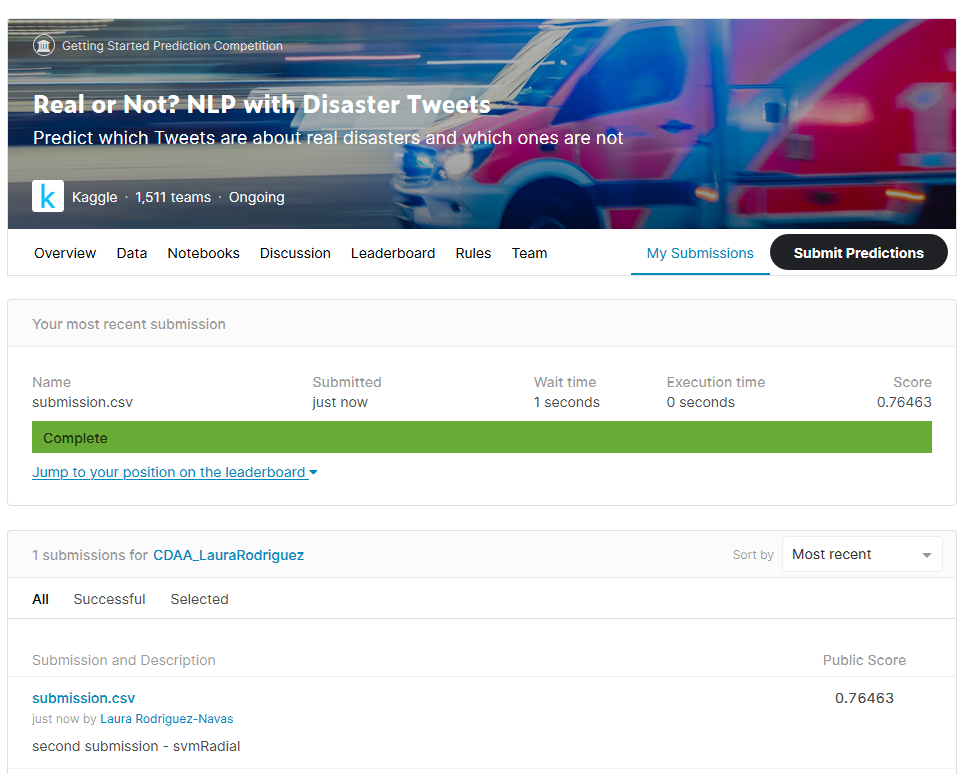
\includegraphics[width=0.8\textwidth,height=\textheight]{submission.png}

\hypertarget{conclusiones}{%
\section{Conclusiones}\label{conclusiones}}

En este documento se revisa cómo importar y preparar documentos de texto
para realizar distintas operaciones de mineria de textos con ellos,
tales como obtener palabras frecuentes, asociaciones de palabras y
análisis de sentimientos.

Si comparamos nuestro resultado con los de los otros usuarios de la
compatición de Kaggle, vemos que el modelo creado no es muy bueno. La
predicción a sido peor de la esperada. Aunque no era la finalidad de
este ejercicio, esto nos demuestra que el ejercicio se podría mejorar en
algunos expectos.

El problema más importante para la realización de este ejercicio ha sido
el coste computacional. Llegado el punto en que la ejecución de todo el
flujo tardaba unas cuantas horas en finalizar, se pensó en utilizar la
computación paralela. Fue una buena idea, se redujo drásticamente el
coste computacional y además aprendí a hacerlo en \textbf{R}.

Personalmente escogí esta competición ya que nunca habia combinado la
clasificación supervisada con Procesamiento del Lenguaje Natural (PLN).
El Procesamiento del Lenguaje Natural dentro de la inteligencia
artificial es un campo que encuentro muy interesante.

Durante la asignatura de Procesamiento del Lenguaje Natural del Máster
no se realiza ninguna pràctica de programación, y me apreció una buena
oportunidad de aprender como aplicar los conocimientos de adquiridos del
Procesamiento del Lenguaje Natural con los conocimientos adquiridos
durante de esta asignatura.

Por supuesto la minería de textos es un área de análisis extensa. Las
siguientes referencias han sido de gran ayuda para realizar este
documento y amplían lo aquí presentado.

\hypertarget{referencias}{%
\section{Referencias}\label{referencias}}

\begin{itemize}
\item
  Machine Learning con R y caret
  \url{https://www.cienciadedatos.net/documentos/41_machine_learning_con_r_y_caret}
\item
  Notebook en Kaggle de barun2104
  \url{https://www.kaggle.com/barun2104/nlp-with-disaster-eda-dfm-svd-ensemble}
\item
  Notebook en Kaggle de sambitmukherjee
  \url{https://www.kaggle.com/sambitmukherjee/bag-of-words-stack-knn-tree-lasso\#test-set-predictions-submission}
\end{itemize}

\end{document}
